% ============================================================
% Curriculum vs Mixed-Batch Training in MARL for Urban Driving
% Tesi di laurea triennale — VERSIONE 2 (italiano, 30 pagine)
%
% Struttura in quattro blocchi:
%   I   Introduzione            (cap. 1)
%   II  Il progetto             (cap. 2–4)
%   III Possibili evoluzioni    (cap. 5)
%   IV  Conclusioni             (cap. 6)
% Frontespizio, sommario, indice, acronimi, appendici e bibliografia
% sono FUORI dal conteggio delle 30 pagine di contenuto.
%
% Build: pdflatex main_it_v2 + biber main_it_v2 + pdflatex x2
%        (oppure: latexmk -pdf main_it_v2)
% ============================================================
\documentclass[12pt,a4paper,oneside]{report}

% --- Encoding & language ---
\usepackage[utf8]{inputenc}
\usepackage[T1]{fontenc}
\usepackage{lmodern}
\usepackage[english,italian]{babel}
\usepackage{csquotes}

% --- Layout ---
\usepackage[a4paper,margin=2.5cm]{geometry}
\usepackage{setspace}
\onehalfspacing
\usepackage{microtype}
% lmtt in T1 ha la legatura "--" -> en-dash: nei blocchi \ttfamily i flag da
% riga di comando (--mode, --difficulty, ...) uscivano come "-mode". La
% disattiviamo per la sola famiglia monospaziata.
\DisableLigatures{encoding = T1, family = tt*}
% Usato nelle colonne p{} strette delle tabelle: la giustificazione su misure
% cosi' corte produce spazi dilatati (29 Underfull \hbox).
\usepackage{ragged2e}
% Ultima risorsa prima di sforare il margine: consente a TeX di allargare gli
% spazi anziche' produrre un Overfull. Non puo' mascherare le scatole
% indivisibili (math inline, \texttt lunghi), che restano segnalate nel log.
\setlength{\emergencystretch}{1.5em}

% --- Math, tables, units, figures ---
\usepackage{amsmath,amssymb}
\usepackage{graphicx}
\graphicspath{{figures/}}
\usepackage{booktabs}
\usepackage{array}
% Colonna a larghezza fissa NON giustificata: su misure di 2--4cm la
% giustificazione apre spazi enormi tra le parole. Sostituisce p{} nelle
% tabelle a colonne strette (3.1, 4.4, A.1, A.2, B.1, C.1).
\newcolumntype{L}[1]{>{\RaggedRight\arraybackslash}p{#1}}
\usepackage{longtable}
\usepackage{verbatim}
\usepackage{siunitx}
\usepackage{tikz}
\usetikzlibrary{positioning,arrows.meta}

% --- Bibliography ---
\usepackage[style=numeric-comp,sorting=none,backend=biber]{biblatex}
\addbibresource{bibliography.bib}
% URL ed eprint in bibliografia erano composti in \ttfamily senza punti di
% rottura: la voce CARLA sforava il margine destro di 16.7pt e l'arXiv id
% 1707.06347 si spezzava dopo il punto. Queste penalita' abilitano le rotture.
\setcounter{biburlnumpenalty}{7000}
\setcounter{biburlucpenalty}{8000}
\setcounter{biburllcpenalty}{7000}

% --- Colors, links, cross-references (hyperref near the end) ---
\usepackage{xcolor}
\usepackage[hidelinks]{hyperref}
\usepackage{xurl}   % dopo hyperref: consente la rottura degli URL lunghi
% Le didascalie occupavano tutta la \textwidth anche sopra oggetti molto piu'
% stretti (fino a 136pt di differenza). Le si restringe leggermente.
\usepackage{caption}
\captionsetup{width=0.90\textwidth}
\usepackage[capitalise,noabbrev]{cleveref}
% Le stringhe italiane di cleveref sono incomplete (niente "chapter") e
% vengono applicate a \begin{document}, sovrascrivendo definizioni date
% nel preambolo. Registriamo quindi le nostre DOPO il suo hook.
\AtBeginDocument{%
  \crefname{chapter}{Capitolo}{Capitoli}%
  \Crefname{chapter}{Capitolo}{Capitoli}%
  \crefname{section}{Sezione}{Sezioni}%
  \Crefname{section}{Sezione}{Sezioni}%
  \crefname{subsection}{Sezione}{Sezioni}%
  \Crefname{subsection}{Sezione}{Sezioni}%
  \crefname{figure}{Figura}{Figure}%
  \Crefname{figure}{Figura}{Figure}%
  \crefname{table}{Tabella}{Tabelle}%
  \Crefname{table}{Tabella}{Tabelle}%
  \crefname{equation}{Equazione}{Equazioni}%
  \Crefname{equation}{Equazione}{Equazioni}%
  \crefname{appendix}{Appendice}{Appendici}%
  \Crefname{appendix}{Appendice}{Appendici}%
}

% I pattern di sillabazione attivi sono italiani e spezzavano male i termini
% inglesi nelle tabelle: "messa-ge", "po-licy".
\hyphenation{mes-sage pass-ing pol-icy batch cur-ric-u-lum base-line}

% --- Note di lavoro: marcatori TODO rossi, rimuovere prima della consegna ---
\newcommand{\todo}[1]{\textcolor{red}{\textbf{[TODO: #1]}}}

% Le tabelle di questa tesi sono dense: si allarga la tolleranza sui
% float per evitare pagine mezze vuote in attesa di collocamento.
\renewcommand{\topfraction}{0.9}
\renewcommand{\bottomfraction}{0.75}
\renewcommand{\textfraction}{0.1}
\renewcommand{\floatpagefraction}{0.8}
\setcounter{topnumber}{3}
\setcounter{bottomnumber}{2}
\setcounter{totalnumber}{4}

% ============================================================
\begin{document}

% Front matter: numeri di pagina romani (il frontespizio conta come i);
% la numerazione araba riparte dal Capitolo 1.
\pagenumbering{roman}

% ----------------- Frontespizio (template ufficiale UniMarconi) --
\begin{titlepage}
  \centering
  
\includegraphics[height=2.0cm]{logo_unimarconi}\par
  \vspace{1.5cm}
  {\large\bfseries UNIVERSIT\`A DEGLI STUDI GUGLIELMO MARCONI\par}
  \vspace{0.9cm}
  {\bfseries DIPARTIMENTO DI INGEGNERIA\par}
  \vspace{0.9cm}
  {\bfseries CORSO DI LAUREA IN INTELLIGENZA ARTIFICIALE (L-8)\par}
  \vfill
  {\Large\itshape ``Curriculum e mixed-batch learning a
  confronto nel Reinforcement Learning multi-agente per la guida
  autonoma in ambiente simulato urbano''\par}
  \vfill
  {\large
   \begin{minipage}[t]{0.50\textwidth}
     \raggedright
     Relatore:\\[1.2em]
     Prof.\ Stefano Aldegheri
   \end{minipage}%
   \hfill
   \begin{minipage}[t]{0.40\textwidth}
     \raggedright
     Candidato:\\[1.2em]
     Fabio Carapelle
   \end{minipage}\par}
  \vfill
  {\footnotesize ANNO ACCADEMICO 2025/2026\par}
\end{titlepage}
% l'ambiente titlepage azzera il contatore; il frontespizio conta come i
\setcounter{page}{2}

% ----------------- Sommario ---------------------------------
\clearpage
\null\vfil
\phantomsection
\addcontentsline{toc}{chapter}{\abstractname}
\begin{center}%
  \bfseries \abstractname
\end{center}
L'ordine in cui i task di addestramento vengono presentati è una
decisione di progetto nel Reinforcement Learning i cui effetti sono
raramente isolati nei contesti multi-agente. Questa tesi confronta il
\emph{curriculum learning} --- progressione dei task da facile, medio 
a difficile, condizionata dalla competenza misurata --- con l'addestramento
\emph{mixed-batch}, che alterna uniformemente tutte le difficoltà fin dall'inizio, 
per la guida autonoma in un contesto urbano simulato (CARLA), con sei agenti 
(tre veicoli e tre pedoni) che apprendono simultaneamente come muoversi in un unico 
mondo condiviso sfruttando l'algoritmo MAPPO ed un critic centralizzato. 
Una campagna $2\times2$ appaiata per seed incrocia i due regimi con due encoder 
del critic (MLP e GNN) a tre milioni di passi per run, su una piattaforma irrobustita 
da un protocollo di sviluppo guidato da gate e misurata con un criterio di successo
rigoroso, con repliche a seed identico a fornire una banda di rumore esplicita.
L'ordinamento dei task non ha accelerato l'apprendimento iniziale: tutte
le celle hanno superato le stesse soglie di competenza agli stessi
conteggi di passi. Ha invece selezionato \emph{che cosa} la policy è
diventata. Con il critic MLP/GNN il curriculum ha prodotto un guidatore
cauto e con più successi, il batch invece uno veloce e incline alle collisioni;
Sul criterio di successo, il curriculum ha prevalso di $+18.5$ punti percentuali ponderati
in valutazione dei veicoli. In entrambe le architetture del critic il curriculum ha prevalso su una città
mai vista in addestramento ($+19.0$ e $+10.0$\,pp). 
I pedoni sono risultati vincolati dalla fattibilità dei percorsi più che dal regime e per questo 
non sono stati tenuti prettamente \enquote{rilevanti} al fine della valutazione, ma sono stati considerati per
evidenziare come diversi attori influenzino gli altri all'interno del mondo usando un criterio di CTDE. 
L'ordinamento dei task, in questo contesto, è un selettore di equilibri il cui beneficio
in-domain dipende dalla stima del valore --- e il cui output più evidente è la generalizzazione ed un tempo di 
esecuzione della run minore a parità di budget a favore del training curriculum.
\par\vfil\null

\tableofcontents

% ----------------- Acronimi ---------------------------------
\chapter*{Acronimi}
\addcontentsline{toc}{chapter}{Acronimi}
% \noindent + colonna a larghezza fissa: con {ll} la riga NPC eccedeva
% \textwidth (Overfull 10.24pt) e usciva nel margine destro.
\noindent\begin{tabular}{@{}l@{\hspace{1.5em}}%
  >{\raggedright\arraybackslash}p{0.78\textwidth}@{}}
CTDE  & Centralized Training with Decentralized Execution \\
GAE   & Generalized Advantage Estimation \\
GNN   & Graph Neural Network \\
MAPPO & Multi-Agent Proximal Policy Optimization \\
MARL  & Multi-Agent Reinforcement Learning \\
MLP   & Multi-Layer Perceptron \\
NPC   & Non-Player Character (partecipante al traffico con comportamento scriptato) \\
PPO   & Proximal Policy Optimization \\
RL    & Reinforcement Learning \\
SR    & Success Rate (tasso di successo) \\
TM    & (CARLA) Traffic Manager \\
\end{tabular}

% ----------------- Corpo della tesi (30 pagine) --------------
\clearpage
\pagenumbering{arabic}

% Blocco I — Introduzione
% ============================================================
% v2 — Capitolo 1: Introduzione
% Blocco I di IV (intro -> progetto -> evoluzioni -> conclusione)
% Budget: ~4 pagine. Include i fondamenti essenziali, ridotti a
% ciò che serve effettivamente nei capitoli successivi.
% ============================================================
\chapter{Introduzione}
\label{ch:intro}

\section{Motivazione e domanda di ricerca}
\label{sec:motivazione}

L'apprendimento per rinforzo (\emph{reinforcement learning}, RL)
addestra politiche di controllo per tentativi ed errori, e in qualunque
dominio non banale il progettista incontra una decisione di scheduling
prima ancora del primo passo di gradiente: quando i task da padroneggiare
coprono un intervallo di difficoltà, \emph{in quale ordine vanno
presentati}? Due risposte sono naturali e opposte. Il \emph{curriculum
learning} li presenta dal facile al difficile, sulla falsariga della
pedagogia umana: si costruisce competenza dove il successo è
raggiungibile, poi la si estende. L'\emph{addestramento misto}
(mixed-batch) li presenta tutti fin dall'inizio, ed è l'analogo diretto
dell'addestramento su un dataset mescolato, default indiscusso
dell'apprendimento supervisionato.

Le due strategie consumano lo stesso budget di calcolo: scegliere tra
loro è, in linea di principio, gratuito. Se la scelta cambia ciò che la
policy appresa fa, allora è tra le leve più economiche a disposizione di
chi progetta un sistema di RL --- ed è anche tra le meno caratterizzate
nei contesti \emph{multi-agente}, dove quasi nessuna delle assunzioni
della letteratura sui curricula (apprendista singolo, reward sparse,
ambiente stazionario) continua a valere.

La guida autonoma urbana è un banco di prova esigente per porre la
domanda: offre un asse di difficoltà naturale e continuo (la lunghezza
del percorso), agenti eterogenei con vincoli fisici diversi, una
tensione strutturale tra prestazione e sicurezza --- le policy più
veloci completano più percorsi \emph{e} urtano più cose --- e un test
out-of-distribution canonico, guidare su una città mai vista in
addestramento. È inoltre intrinsecamente multi-agente: le policy non si
limitano a condividere un mondo, ma plasmano l'ambiente l'una
dell'altra mentre apprendono.

\begin{quote}
  \emph{Il curriculum learning da easy a medium a hard produce un
  comportamento di guida multi-agente misurabilmente diverso rispetto
  all'addestramento mixed-batch, a parità di budget di addestramento?}
\end{quote}

La domanda riguarda deliberatamente il \emph{comportamento} e non una
singola classifica di tassi di successo: il confronto è valutato lungo
quattro assi --- efficienza campionaria iniziale, prestazione finale con
la sua composizione dei fallimenti, dinamica entro la run e
generalizzazione a una mappa nuova --- sempre separando veicoli e
pedoni. Tre ipotesi falsificabili strutturano l'analisi:

\begin{itemize}
  \item \textbf{H1 (curriculum).} L'esposizione graduale produce una
        migliore efficienza campionaria iniziale, perché i task facili
        offrono successi raggiungibili da cui partire; con il rischio
        noto di plateau od oblio sui task difficili introdotti tardi.
  \item \textbf{H2 (misto).} L'esposizione uniforme copre l'intera
        distribuzione dei task dal passo zero, al costo di un segnale
        iniziale più rumoroso; il suo payoff atteso è la robustezza.
  \item \textbf{H3 (interazione, secondaria).} L'entità --- forse la
        direzione --- dell'effetto di regime può dipendere da come viene
        stimato il valore: nelle architetture ad addestramento
        centralizzato è il \emph{critic} a digerire la struttura
        multi-agente, e sostituirne l'encoder può cambiare ciò che
        l'ordinamento produce.
\end{itemize}

\section{Fondamenti essenziali}
\label{sec:fondamenti}

Questa sezione introduce solo i concetti effettivamente usati nel
seguito, ciascuno alla profondità alla quale serve.

\paragraph{RL, valore e vantaggio.}
Il RL formalizza la decisione sequenziale come processo decisionale di
Markov $(\mathcal{S}, \mathcal{A}, P, r, \gamma)$~\cite{sutton2018rl}:
un agente agisce tramite una policy $\pi(a \mid s)$ e massimizza il
ritorno atteso scontato
$J(\pi) = \mathbb{E}_{\pi}[\sum_{t \geq 0} \gamma^{t} r(s_t,a_t)]$. Lo
sconto fissa un orizzonte decisionale effettivo di $\approx 1/(1-\gamma)$
passi: non è una costante cosmetica, perché la piattaforma del
\cref{ch:piattaforma} usa $\gamma = 0.997$, cioè $\approx 333$ passi, su
episodi lunghi fino a mille passi. Il \emph{vantaggio}
$A^{\pi}(s,a) = Q^{\pi}(s,a) - V^{\pi}(s)$ misura quanto un'azione sia
migliore della media della policy in quello stato, e il teorema del
gradiente di policy fornisce
$\nabla_{\theta} J = \mathbb{E}_{\pi_\theta}[\nabla_{\theta}\log\pi_{\theta}(a_t\mid s_t)\,A^{\pi}(s_t,a_t)]$.
Poiché stimare $A$ con ritorni Monte Carlo grezzi produce alta varianza,
si sottrae una baseline appresa: i metodi \emph{actor--critic}
addestrano perciò l'actor $\pi_\theta$ e il critic $V_\phi$ --- e questa
divisione del lavoro è l'aggancio all'architettura multi-agente, perché
il critic è un dispositivo del solo addestramento e può quindi ricevere
informazione che l'actor non vede mai.

\paragraph{PPO, GAE ed entropia.}
Gli aggiornamenti di gradiente ``vanilla'' sono fragili, perché un
singolo passo troppo grande può far collassare una policy funzionante.
PPO~\cite{schulman2017ppo} lo evita con un obiettivo surrogato clippato:
detto $\rho_t(\theta) = \pi_{\theta}(a_t\mid s_t)/\pi_{\theta_{\text{old}}}(a_t\mid s_t)$
il rapporto di importanza,
\begin{equation}
  L^{\mathrm{CLIP}}(\theta) =
  \mathbb{E}_t\!\left[\min\bigl(\rho_t A_t,\;
  \operatorname{clip}(\rho_t,\, 1-\varepsilon,\, 1+\varepsilon)\, A_t\bigr)\right],
\end{equation}
il che rimuove ogni incentivo a spostare il rapporto oltre
$[1-\varepsilon, 1+\varepsilon]$ e permette più epoche di gradiente su
ogni batch senza aggiornamenti distruttivi. I vantaggi $A_t$ provengono
da GAE~\cite{schulman2016gae}, che con i residui temporali
$\delta_t = r_t + \gamma V(s_{t+1}) - V(s_t)$ pone
$A_t = \sum_{l \geq 0} (\gamma\lambda)^{l}\delta_{t+l}$, dove $\lambda$
scambia bias e varianza tra il TD a un passo e i ritorni Monte Carlo, e
la cui qualità dipende direttamente da quella del critic. Un bonus di
entropia sostiene infine l'esplorazione penalizzando il collasso
prematuro della policy.

\paragraph{MARL, CTDE e MAPPO.}
Con $N$ agenti in un unico ambiente l'MDP si generalizza a un
\emph{gioco di Markov}, e sorgono due difficoltà strutturali. La prima è
la \emph{non-stazionarietà}: dal punto di vista di ciascun agente gli
altri sono parte dell'ambiente e stanno apprendendo, quindi la dinamica
effettiva cambia nel tempo e l'esperienza raccolta sotto vecchie policy
dei co-giocatori diventa fuorviante~\cite{lowe2017maddpg}. La seconda è
l'\emph{attribuzione del merito}: il ritorno di ogni agente dipende
dalle azioni di tutti. La risoluzione ormai standard sfrutta la
divisione actor--critic: si addestrano i critic con accesso a
informazione globale, mantenendo gli actor condizionati sulle sole
osservazioni locali~\cite{lowe2017maddpg}. Il critic assorbe la
non-stazionarietà, mentre l'esecuzione resta pienamente decentralizzata
perché i critic vengono scartati dopo l'addestramento: è il paradigma
\emph{centralized training, decentralized execution} (CTDE), usato in
tutta questa tesi. MAPPO~\cite{yu2022surprising} lo istanzia con actor
PPO e funzione di valore centralizzata, e Yu et al.\ mostrano che questa
combinazione minimale eguaglia o supera i metodi off-policy sui
benchmark cooperativi standard purché i dettagli implementativi siano
corretti --- fra i quali proprio il design dell'input del critic. Nel
critic più semplice quell'input è la concatenazione piatta delle
osservazioni di tutti gli agenti; le alternative strutturate le trattano
come nodi di un grafo, ed è il confronto tra queste due famiglie a
costituire l'asse secondario di questa tesi (\cref{sec:critic}).

\paragraph{Curriculum learning e la sua condizione di controllo.}
L'idea che l'apprendimento migliori quando gli esempi sono presentati in
un ordine sensato precede il deep learning: gli esperimenti
\emph{starting small} di Elman mostrarono reti ricorrenti capaci di
apprendere una grammatica complessa solo quando la complessità
dell'input cresceva incrementalmente~\cite{elman1993starting}, e Bengio
et al.~\cite{bengio2009curriculum} diedero poi alla strategia il nome di
curriculum learning, inquadrandola come metodo di continuazione in cui
gli esempi facili definiscono una versione più liscia dell'obiettivo.
Nel RL il progettista controlla non solo
l'ordine dei dati ma la distribuzione dei \emph{task}, il che rende i
curricula al tempo stesso più potenti e più difficili da progettare;
nella tassonomia della survey di Narvekar et
al.~\cite{narvekar2020curriculum} il meccanismo della \cref{sec:regimi}
è uno schema di \emph{sequenziamento} basato sulla prestazione su un
insieme fisso di task. La motivazione riguarda in larga parte
l'esplorazione: sui task difficili una policy debole può non
sperimentare praticamente mai il successo, e quindi non ricevere segnale
di apprendimento. Tre modi di fallimento noti hanno plasmato il design
del \cref{ch:piattaforma} --- l'\emph{oblio} della competenza precedente
sotto distribuzione spostata~\cite{french1999catastrophic}, lo
\emph{stallo} su un gate mai soddisfatto e la \emph{mis-calibrazione}
del gate stesso --- e sono esattamente i rischi che H1 mette alla prova.
Ogni affermazione sull'ordinamento richiede però una baseline in cui
esso è \emph{assente}, ed è la condizione che il braccio batch
implementa.

\paragraph{Il simulatore CARLA.}
CARLA~\cite{dosovitskiy2017carla} è un simulatore open-source di guida
urbana su Unreal Engine~4, distribuito come server che ospita mondo e
fisica e pilotato da client via API Python. Conta qui per tre ragioni
(versione 0.9.16 ovunque): la \emph{modalità sincrona a passo fisso}
rende la raccolta di esperienza indipendente dal rendering; i pedoni
sono attori \emph{walker} ad azionamento diretto, il che rende possibile
apprenderne le policy; e le città fornite differiscono \emph{in natura}
e non solo in dimensione --- l'addestramento usa \emph{Town03}, ``a
larger, urban map with a roundabout and large junctions'', il test di
generalizzazione \emph{Town05}, una ``squared-grid town with cross
junctions and a bridge'' a più corsie per direzione~\cite{carladocs}.
Anche in modalità sincrona e con tutti i seed fissati, infine, CARLA
sotto carico multi-agente non è deterministico da run a run: una
variabilità irriducibile quantificata e usata come metro per ogni
effetto riportato (\cref{sec:gate}).

\section{Approccio, contributi e struttura}
\label{sec:approccio}

Tutti gli esperimenti girano su Town03, con Town05 riservata al solo
test di generalizzazione. Sei agenti apprendono simultaneamente in un
unico mondo condiviso --- tre veicoli e tre pedoni, ciascuno con un
percorso proprio a ogni episodio --- un design che chiamiamo
\emph{copertura parallela dei task} e che è la cornice fissa di entrambi
i bracci sperimentali, non una variabile. Le policy sono addestrate con
MAPPO in regime CTDE, con una policy condivisa per classe e un critic
centralizzato che vede le osservazioni di tutti gli agenti solo durante
l'addestramento; la difficoltà è la lunghezza target del percorso
(30/60/\SI{100}{m}) e il successo è il completamento rigoroso del
percorso assegnato.

I due regimi condividono ogni componente tranne la regola di selezione
del livello: il braccio \emph{curriculum} parte dal solo easy e sblocca
i livelli successivi attraverso un gate di competenza a finestra, il
braccio \emph{batch} alterna uniformemente tutti i livelli fin dal primo
episodio. La campagna finale è un fattoriale $2 \times 2$ --- \{critic
MLP, critic GNN\} $\times$ \{curriculum, batch\} --- di quattro run da
tre milioni di passi a seed singolo appaiato, ciascuna seguita da una
valutazione di 400 episodi che include Town05. Con una run per cella
ogni contrasto è un caso di studio appaiato, letto contro una banda di
varianza misurata su repliche a seed identico; il contrasto primario è
però osservato \emph{due volte}, una per architettura del critic.
Anticipando il \cref{ch:risultati}: la clausola di efficienza di H1 e
quella di robustezza di H2 falliscono entrambe, mentre H3 regge in forma
forte.

I contributi sono quattro: \textbf{(i)} un framework di confronto
controllato a parità di budget, con run appaiate per seed e regole di
misura rigorose per agente; \textbf{(ii)} una metodologia di sviluppo
guidata da gate con un registro onesto di modifiche promosse, rigettate
e consapevolmente mantenute, in cui i difetti di validità dell'ambiente
--- incluso uno che ha spostato la metrica principale di $\approx 50$
punti percentuali senza alcun cambiamento di policy --- sono documentati
con le loro firme di rilevamento; \textbf{(iii)} una caratterizzazione
empirica di che cosa fa l'ordinamento dei task, ossia nessun effetto di
efficienza iniziale ma selezione tra equilibri di guida
qualitativamente diversi; e \textbf{(iv)} l'evidenza che gli effetti di
regime sono condizionati dalla stima del valore.

La tesi prosegue in quattro blocchi. I
\cref{ch:piattaforma,ch:metodo,ch:risultati} descrivono il progetto:
rispettivamente la piattaforma sperimentale, il metodo di misura con il
design della campagna, e i risultati con la loro interpretazione. Il
\cref{ch:evoluzioni} raccoglie le possibili evoluzioni del lavoro e il
\cref{ch:conclusioni} conclude.


% Blocco II — Il progetto
% ============================================================
% v2 — Capitolo 2: Il progetto — la piattaforma sperimentale
% Blocco II di IV. Budget: ~7 pagine.
% Fonti verificate da codice (invariate rispetto alla v1):
%   carla_multi_agent_env.py, route_planner.py,
%   curriculum_batch_manager.py, centralized_critic.py,
%   train_mappo.yaml, curriculum_batch.yaml, levels.yaml.
% ============================================================
\chapter{Il progetto --- la piattaforma sperimentale}
\label{ch:piattaforma}

Questo capitolo descrive la piattaforma su cui poggia l'esperimento: un
ambiente di apprendimento per rinforzo multi-agente costruito su CARLA,
in cui tre veicoli e tre pedoni sono addestrati congiuntamente con l'algoritmo
MAPPO sotto due regimi alternativi --- curriculum e mixed-batch --- che
condividono ogni altro componente dello stack. L'obiettivo di design è
che il regime sia l'\emph{unica} variabile indipendente
dell'esperimento: tutto ciò che è documentato qui è comune a entrambi i
bracci, e la \cref{sec:regimi} isola il punto esatto in cui divergono.

% ------------------------------------------------------------
\section{Panoramica dell'architettura}
\label{sec:architettura}

La piattaforma consiste di quattro strati (\cref{fig:architettura}).
Il \textbf{simulatore} è CARLA 0.9.16, che gira come server autonomo
pilotato in modalità sincrona con passo di fisica fisso di \SI{0.05}{s}
(\SI{20}{Hz}): avanza solo quando l'ambiente emette un tick, il che
rende la raccolta di esperienza deterministica rispetto allo scheduling.
Il traffico scriptato non apprendente --- 15 veicoli e 30 pedoni NPC in
ogni livello --- è gestito dal Traffic Manager, anch'esso sincrono.
L'\textbf{ambiente multi-agente} (\texttt{CarlaMultiAgentEnv}) espone la
simulazione a RLlib come interfaccia multi-agente con sei agenti
apprendenti: a ogni reset spawna gli agenti, assegna a ciascuno un
percorso individuale (\cref{sec:percorsi}) e configura lo scenario
secondo il livello selezionato dal manager curriculum/batch
(\cref{sec:regimi}); un episodio dura al più 1000 passi di controllo,
cioè \SI{50}{s} di tempo simulato.

Lo \textbf{stack di apprendimento} è MAPPO su Ray/RLlib 2.10.0 con
PyTorch 2.7. Vengono apprese due policy, una condivisa dai tre veicoli e
una dai tre pedoni --- condivisione di parametri entro ciascuna classe,
nessuna condivisione tra classi, poiché le due hanno spazi di
osservazione e azione diversi. Ogni actor è un percettrone multistrato
con due strati nascosti da 256 unità; un critic centralizzato riceve
un'osservazione globale a 225 dimensioni che concatena informazione per
agente (\cref{sec:osservazioni}), con encoder MLP di default e una
variante a grafo come asse sperimentale secondario (\cref{sec:critic}).
Infine il \textbf{logging}: alla fine di ogni episodio il processo di
addestramento accoda un record JSON \emph{per agente} --- sei per
episodio --- a un file \texttt{episodes.jsonl} contenente ragione di
terminazione, completamento ed efficienza del percorso, velocità e
diagnostica di generazione del percorso. Tutti i risultati del
\cref{ch:risultati} sono calcolati da questi record.

\begin{figure}[t]
  \centering
  \begin{tikzpicture}[
      node distance=5mm and 10mm,
      box/.style={draw, rounded corners=2pt, align=center,
                  minimum width=48mm, minimum height=9mm, font=\small},
      lbl/.style={font=\scriptsize, midway},
      >={Stealth[length=2.5mm]}]
    \node[box] (carla) {Server CARLA 0.9.16\\ \scriptsize Town03 (train) / Town05 (test), TM};
    \node[box, below=of carla] (env) {\texttt{CarlaMultiAgentEnv}\\ \scriptsize 3 veicoli + 3 walker, route planner};
    \node[box, right=of env] (mgr) {Manager curriculum\\ / batch \scriptsize (livello per episodio)};
    \node[box, below=of env] (rllib) {Ray/RLlib 2.10 --- MAPPO (CTDE)\\ \scriptsize policy veicolo, policy pedone, critic centralizzato};
    \node[box, below=of rllib] (log) {\texttt{episodes.jsonl}\\ \scriptsize 6 record/episodio};
    \node[box, right=of log] (eval) {Pipeline di valutazione\\ \scriptsize $4$ scenari $\times$ 100 ep};
    \draw[->] (env) -- node[lbl, right] {tick / controllo} (carla);
    \draw[<-] ([xshift=-8mm]env.north) -- node[lbl, left] {sensori, stato} ([xshift=-8mm]carla.south);
    \draw[->] (mgr) -- node[lbl, above] {livello} (env);
    \draw[->] (env) -- node[lbl, right] {oss., reward} (rllib);
    \draw[<-] ([xshift=-8mm]env.south) -- node[lbl, left] {azioni} ([xshift=-8mm]rllib.north);
    \draw[->] (rllib) -- (log);
    \draw[->] (rllib) -| node[lbl, above, pos=0.25] {checkpoint} (eval);
  \end{tikzpicture}
  \caption{Architettura a componenti. Il manager curriculum/batch è
  l'unico componente che differisce tra i due bracci sperimentali, e
  solo nella regola di selezione del livello (\cref{sec:regimi}).}
  \label{fig:architettura}
\end{figure}

% ------------------------------------------------------------
\section{Un mondo condiviso: la copertura parallela dei task}
\label{sec:mondo}

I sei agenti apprendenti non cooperano verso un obiettivo congiunto: a
ciascuno è assegnato il \emph{proprio} percorso ed è valutato
individualmente sul suo completamento. Poiché tutti e sei i percorsi
sono collocati nello stesso mondo vivo, un singolo episodio esercita
simultaneamente sei micro-task diversi --- geometrie stradali diverse,
interazioni diverse con il traffico scriptato e, soprattutto,
interazioni reciproche tra agenti apprendenti, per esempio un veicolo
che dà la precedenza a un pedone anch'esso in addestramento. Chiamiamo
questo design \emph{copertura parallela dei task}: per episodio di
orologio il sistema raccoglie esperienza su sei istanze di task anziché
una. Rispetto ai benchmark cooperativi che motivano MAPPO, il setting è
meglio descritto come \emph{coesistenza} di task indipendenti in un
mondo condiviso --- nessuna reward di squadra, nessuna competizione
esplicita, ma un accoppiamento reale attraverso lo stato del mondo.

Ne seguono due avvertenze. Primo, i sei campioni per episodio sono
\emph{correlati}, perché gli agenti condividono lo stato del mondo: per
questo il \cref{ch:metodo} non usa mai i conteggi di record come se
fossero osservazioni indipendenti. Secondo, dal punto di vista di ogni
singolo agente l'ambiente è \emph{non-stazionario} durante
l'addestramento, perché le policy degli altri cinque cambiano nel tempo
--- la motivazione standard del critic CTDE. La copertura parallela
resta comunque una proprietà della piattaforma, identica in entrambi i
regimi: parte della cornice sperimentale, non una variabile.

\paragraph{Percorsi per agente e seeding.}
A ogni reset ciascun agente riceve un percorso indipendente la cui
lunghezza target è fissata dal livello attivo. La generazione ha un seed
deterministico per agente con una sequenza costruita da:

$\langle\text{seed traffico},\ \text{contatore di reset},\
\mathrm{crc32}(\text{id agente})\rangle$

cosicché due run lanciate con lo stesso seed sullo stesso codice vedano 
la stessa sequenza di estrazioni e le estrazioni siano disaccoppiate tra 
agenti. È questa proprietà a rendere i confronti A/B appaiati \emph{per costruzione}, 
e su di essa il protocollo del \cref{ch:metodo} fa affidamento.

\paragraph{Tassonomia delle terminazioni.}
Ogni agente termina il proprio episodio in modo indipendente con
esattamente una di sei ragioni: \texttt{route\_complete} (l'\emph{unico}
esito contato come successo); \texttt{route\_short}, cioè la fine di un
percorso risultato più corto del target oltre una tolleranza --- un
fallback degenere che \emph{non} conta come successo, così da prevenire
l'inflazione della metrica tramite percorsi banalmente brevi;
\texttt{collision}; \texttt{offroad} (il veicolo si è spostato più di
\SI{5}{m} dal centro della corsia più vicina); \texttt{stuck} (mancanza
prolungata di progresso); e \texttt{timeout}. Ogni episodio produce
quindi esattamente sei record a livello di agente.

% ------------------------------------------------------------
\section{Spazi di osservazione e azione}
\label{sec:osservazioni}

Ogni agente riceve un vettore di osservazione compatto e specifico per
classe, con tutte le componenti normalizzate in $[-1,1]$ e sanificate
contro valori non finiti: 47 dimensioni per i veicoli, 26 per i pedoni
(\cref{tab:obs}). Il design architetturale è strutturato come segue:
cinematica dell'ego e dei vicini più prossimi, in cui entrambe le
classi osservano una breve \emph{anteprima} del proprio percorso ---
offset relativi dei waypoint successivi nel riferimento dell'ego ---
insieme all'errore di heading e, per i veicoli, all'angolo della curva
imminente: la geometria locale del task assegnato, senza nulla degli
obiettivi altrui. In secondo luogo, una routine condivisa stima lungo il
corridoio frontale un rischio di time-to-collision e una frazione di
occupazione, calcolati separatamente contro i veicoli (corridoio
\SI{3.5}{m}, \SI{40}{m} avanti, orizzonte \SI{5}{s}) e contro i pedoni
(\SI{3.0}{m}, \SI{30}{m}, \SI{4}{s}); gli stessi quattro valori lato
veicolo sono riusati dalla reward come gate di sicurezza
(\cref{sec:reward}), così che la quantità che modula la reward sia
\emph{sempre} visibile alla policy. Infine, le ultime tre dimensioni del
veicolo espongono stato interno dell'ambiente da cui la reward dipende
--- passi senza progresso, penalità anti-loop e tempo rimanente ---
senza le quali le penalità agirebbero su informazione che l'agente non
può osservare, un difetto di aliasing di stato identificato e corretto
durante lo sviluppo (\cref{sec:gate}).

\paragraph{Spazi di azione.}
Entrambe le classi usano azioni continue bidimensionali. L'azione del
veicolo è $[a_{\mathrm{tb}}, a_{\mathrm{steer}}] \in [-1,1]^2$, dove
$a_{\mathrm{tb}}$ positivo mappa sull'acceleratore e negativo sul freno;
quella del pedone è $[a_{\mathrm{speed}}, a_{\Delta\mathrm{h}}]$, con
$a_{\mathrm{speed}} \in [0,1]$ che scala una velocità massima di
camminata di \SI{5.0}{m/s} e $a_{\Delta\mathrm{h}} \in [-1,1]$ che
comanda un cambio di heading fino a $\pm 45^{\circ}$ per passo. Per il
controllo continuo la policy è una gaussiana diagonale: il campionamento
non è un dettaglio implementativo ma parte dell'oggetto appreso, un
punto che diventerà concreto nella \cref{sec:validita}.

\paragraph{Osservazione globale per il critic.}
Durante il solo addestramento il critic riceve una concatenazione a slot
fissi delle osservazioni di tutti gli agenti seguita da una maschera di
vitalità:
$[\,v_0\,|\,v_1\,|\,v_2\,|\,p_0\,|\,p_1\,|\,p_2\,|\,\text{alive}_{6}\,]$,
cioè $3 \times 47 + 3 \times 26 + 6 = 225$ dimensioni. La maschera è
necessaria perché gli agenti terminano in modo indipendente: gli slot di
quelli terminati vengono mascherati anziché riusati silenziosamente. Gli
actor non vedono mai questo vettore, preservando l'esecuzione
decentralizzata.

% ------------------------------------------------------------
\section{Design della reward}
\label{sec:reward}

Le reward sono per agente e identiche nei due regimi; la
\cref{tab:reward} elenca ogni componente con trigger e ampiezza, e la
forma finale è l'esito delle iterazioni guidate da gate documentate
nella \cref{sec:gate} --- nessuna pretesa di ottimalità è attribuita ai
singoli coefficienti. Per entrambe le classi il segnale dominante è un
bonus sparso per waypoint raggiunto, completato da uno shaping denso
proporzionale alla riduzione per passo della distanza dal waypoint
successivo, con i waypoint saltati penalizzati così che il progresso non
sia manipolabile con scorciatoie.

Il blocco empiricamente più delicato è lo \textbf{shaping anti-stallo
condizionato all'hazard}, che contrasta l'\emph{equilibrio difensivo} in
cui un veicolo si ferma indefinitamente per evitare qualunque rischio.
Tutti i suoi termini sono sospesi mentre il veicolo attende
legittimamente a un semaforo rosso o giallo. Lo scalare
$\mathit{hazard} = \max(\text{TTC}_{\mathrm{veh}}, \text{occ}_{\mathrm{veh}},
\text{TTC}_{\mathrm{ped}}, \text{occ}_{\mathrm{ped}})$ riassume il canale
di anteprima della \cref{sec:osservazioni}, e un booleano
$\mathit{safe\_to\_push} = (\mathit{hazard} < 0.85)$ fa da gate ai
termini di spinta: una penalità di inattività sotto 2.5~km/h; un bonus
di partenza proporzionale ad acceleratore, allineamento e a un fattore
di urgenza crescente con il tempo trascorso senza progresso; e uno
shaping di velocità minima attorno a un target di 8~km/h. Sopra la
soglia di hazard ogni incentivo di spinta scompare, quindi la policy non
è mai premiata per accelerare in un corridoio rischioso;
indipendentemente dal gate, una rampa di non-progresso e una penalità
anti-loop rendono lo stallo prolungato e il girare in tondo strettamente
non redditizi.

I pedoni, infine, guadagnano un bonus per passo mentre camminano entro
una \textbf{banda di comfort} di $[1.2, 2.6]$~m/s, intenzionalmente
ampia: a 2.0~m/s un pedone copre \SI{100}{m} --- il target del livello
hard --- entro l'orizzonte di \SI{50}{s}. Il suo design asimmetrico
(solo bonus) e la sua interazione con il gate di hazard dei veicoli sono
un caso concreto di accoppiamento tra classi, analizzato empiricamente
nel \cref{ch:risultati}.

% ------------------------------------------------------------
\section{Generazione dei percorsi e livelli di difficoltà}
\label{sec:percorsi}

La difficoltà è definita dalla \emph{lunghezza target} dei percorsi per
agente, con tutti gli altri parametri di scenario tenuti costanti: i tre
livelli di addestramento collocano i target di veicoli e pedoni a 30
(easy), 60 (medium) e \SI{100}{m} (hard), sempre su Town03 e sempre con
lo stesso traffico scriptato; un quarto livello di sola valutazione
(\emph{test}) usa Town05 con target di \SI{80}{m}.

I percorsi dei veicoli sono pianificati sulla topologia stradale con il
global route planner di CARLA: le destinazioni candidate sono campionate
attorno alla distanza target e accettate solo se la lunghezza del
cammino ottimo ricade in $[0.5, 2.0] \times$ il target, con fino a 32
tentativi per reset; se nessuna sopravvive, l'ambiente ripiega su un
generatore legacy a catena di waypoint. I percorsi dei pedoni sono
invece catene di segmenti di marciapiede connesse attraverso
attraversamenti pedonali, plasmate da due vincoli: le catene sotto
$0.5 \times$ il target vengono rigettate --- la stessa guardia che
sostiene la retrocessione \texttt{route\_short} --- e gli
attraversamenti per percorso sono limitati a tre, un tetto
all'esposizione sulla carreggiata fissato empiricamente
(\cref{sec:gate}). La fattibilità dei percorsi pedonali su Town03 è una
\emph{limitazione strutturale} della piattaforma --- la topologia dei
marciapiedi spesso non può sostenere i target nominali medium e hard ---
ed è analizzata nella \cref{sec:pedoni}.

% ------------------------------------------------------------
\section{I due regimi di addestramento}
\label{sec:regimi}

Il regime è la variabile indipendente dell'esperimento principale.
Entrambi sono implementati dallo stesso componente manager, consultato
una volta per reset per selezionare il livello; condividono le
definizioni di livello della \cref{sec:percorsi}, il budget totale di
$3 \times 10^6$ passi d'ambiente e ogni altro componente descritto in
questo capitolo. Differiscono \emph{solo} nella regola di selezione.

\paragraph{Braccio curriculum: progressione condizionata alla competenza.}
L'addestramento parte con il solo livello easy sbloccato. I livelli
superiori si sbloccano attraverso un gate di competenza valutato su una
finestra scorrevole degli ultimi 50 episodi: il tasso di successo a
finestra è calcolato separatamente per la policy veicolo e per quella
pedone, e il gate vincola sul \emph{minimo} dei due --- la progressione
richiede che la classe più debole sia competente, non la media. Medium
si sblocca a un tasso di successo a finestra di almeno il 70\%, hard al
60\%; la finestra deve essere piena, e una quota minima del budget deve
già essere stata spesa ai livelli precedenti (20\% su easy prima di
medium, 28\% su medium prima di hard). Due decisioni di design meritano
giustificazione. La prima è il gating \emph{a finestra} e non
cumulativo: il tasso cumulativo è un integratore in ritardo, trascinato
verso il basso dai fallimenti di avvio a freddo, e una policy può essere
competente \emph{adesso} mentre la sua media dalla nascita è ancora ben
sotto soglia. La seconda sono i \emph{cap di pressione}: se una soglia
non viene mai raggiunta, il livello si sblocca comunque una volta
consumata una quota fissa del budget (30\% per medium, 70\% per hard),
così che il braccio curriculum non possa fermarsi e terminalmente su easy.
Una volta sbloccati, i livelli sono campionati con pesi che normalizzano
a $0.30/0.35/0.35$, e quelli appena sbloccati passano per una breve fase
di \emph{probation} a pressione ridotta (\cref{fig:fsm}).

\paragraph{Braccio batch: alternanza stratificata.}
Il braccio mixed-batch è il \emph{controllo senza ordinamento}: tutti e
tre i livelli sono disponibili dal primo episodio, campionati per
mescolamento stratificato senza reinserimento con finestra --- ogni
finestra consecutiva di tre episodi è una permutazione uniformemente
casuale di \{easy, medium, hard\}. Ne risulta esposizione uniforme
$1/3$ con sbilanciamento massimo di un episodio per campionatore,
evitando sia la deriva del campionamento i.i.d.\ sia qualunque
ordinamento deterministico fisso.


\begin{figure}[t]
  \centering
  \begin{tikzpicture}[
      state/.style={draw, rounded corners=2pt, align=center,
                    minimum width=31mm, minimum height=11mm, font=\small},
      gate/.style={font=\scriptsize, align=center},
      >={Stealth[length=2.5mm]}, node distance=15mm]
    \node[state] (s1) {solo easy\\ \scriptsize campionamento: easy 1.0};
    \node[state, right=of s1] (s2) {easy $+$ medium\\ \scriptsize probation, poi\\ \scriptsize $\propto 0.30/0.35$};
    \node[state, right=of s2] (s3) {easy $+$ medium $+$ hard\\ \scriptsize probation (hard $\times$0.85), poi\\ \scriptsize $\propto 0.30/0.35/0.35$};
    \draw[->] (s1.north east) to[bend left=26]
      node[gate, above] {SR fin.\ $\geq 0.70$\\ $\wedge$ quota easy $\geq 0.20$} (s2.north west);
    \draw[->, dashed] (s1.south east) to[bend right=26]
      node[gate, below] {cap: 30\% budget} (s2.south west);
    \draw[->] (s2.north east) to[bend left=26]
      node[gate, above] {SR fin.\ $\geq 0.60$\\ $\wedge$ quota med.\ $\geq 0.28$} (s3.north west);
    \draw[->, dashed] (s2.south east) to[bend right=26]
      node[gate, below] {cap: 70\% budget} (s3.south west);
  \end{tikzpicture}
  \caption{Progressione del curriculum. Archi pieni: gate di competenza
  sul tasso di successo a finestra (minimo sulle due policy, finestra di
  50 episodi piena) con soglie minime di quota di budget. Archi
  tratteggiati: cap di pressione che garantiscono la progressione entro
  il budget.}
  \label{fig:fsm}
\end{figure}


Sotto questa costruzione i due bracci consumano lo stesso budget sulla
stessa distribuzione di task in attesa; ciò che differisce è
\emph{quando} ogni parte di quella distribuzione viene presentata, e se
la presentazione è condizionata alla competenza misurata. Qualunque
differenza comportamentale è quindi attribuibile alla politica di
ordinamento, a meno della varianza da run a run --- quantificata nella
\cref{sec:gate} e discussa nella \cref{sec:minacce}.

% ------------------------------------------------------------
\section{Encoder del critic, ottimizzazione e valutazione}
\label{sec:critic}

Nella configurazione di default il critic centralizzato è un MLP che
mappa l'osservazione globale a 225 dimensioni attraverso due strati
nascosti da 256 unità verso un valore scalare. L'asse sperimentale
secondario sostituisce questo encoder con uno su grafo, mentre
\emph{entrambi gli actor restano gli identici MLP} della
\cref{sec:architettura}: qualunque differenza comportamentale tra le due
varianti è quindi attribuibile alla stima del valore durante
l'addestramento e non alla capacità della policy, e a tempo di
esecuzione le due varianti sono indistinguibili. L'encoder GNN riseziona
l'osservazione globale nei sei slot per agente, proietta ciascuno
attraverso uno strato lineare per classe in un embedding di nodo a 64
dimensioni e applica due round di message passing con aggregazione a
media in stile GraphSAGE~\cite{hamilton2017graphsage}: ogni nodo combina
il proprio embedding con la media degli embedding degli altri agenti
\emph{vivi}, e un mean-pool mascherato produce l'input della testa di
valore. La maschera di vitalità guida aggregazione e pooling, così che
gli agenti terminati escano dal riassunto del critic invece di
contribuire slot stantii. La codebase fornisce anche un encoder ad
attenzione e la normalizzazione PopArt dietro flag (entrambi disabilitati 
e lasciati come finetuning futuro)

\paragraph{Ottimizzazione.}
Tutte le run della campagna condividono la stessa configurazione,
byte-identica tra i bracci salvo i flag di regime ed encoder: learning
rate $5\times10^{-4}$; $\gamma = 0.997$; GAE $\lambda = 0.95$; clip PPO
$\varepsilon = 0.2$ con penalità KL aggiuntiva; batch di addestramento
8{.}000 passi, minibatch 256, 15 epoche SGD per batch. Il coefficiente
di entropia segue uno schedule da 0.03 a 0.005 ancorato all'83\% del
budget, espresso come frazione così che run diagnostiche brevi e run
complete attraversino lo stesso profilo di esplorazione. La
configurazione completa è nell'\cref{app:config}.

\paragraph{Pipeline di valutazione.}
I risultati sono misurati a tre livelli, tutti calcolati dai record a
livello di agente. Il \emph{flusso di addestramento} fornisce le
metriche cumulative su tutti gli episodi: sono on-policy e, nel braccio
curriculum, calcolate su un mix di livelli che cambia nel tempo, quindi
caratterizzano il processo di addestramento e non l'abilità finale. Il
\emph{ricalcolo statico} è un passaggio offline che ricalcola gli
aggregati da disco, deduplica i record e verifica l'integrità. La
\emph{valutazione finale del checkpoint} ricarica il modello addestrato
e lo esegue su quattro scenari fissi da 100 episodi ciascuno --- easy,
medium e hard su Town03, più il livello test su Town05 --- ed è l'unico
confronto a distribuzione appaiata tra i bracci; gli episodi sono
valutati con la policy \emph{stocastica}, con re-seeding per episodio
dello scenario e del campionatore di azioni, perché valutare la media
deterministica collasserebbe la policy su una singola traiettoria per
scenario (\cref{sec:validita}).

% ============================================================
% v2 — Capitolo 3: Il progetto — metodo e campagna
% Blocco II di IV. Budget: ~4 pagine.
% Include, condensati: regole di misura, protocollo a gate,
% i tre episodi di validità dell'ambiente (con il pilota di aprile
% ridotto a un paragrafo) e il design della campagna 2x2.
% ============================================================
\chapter{Il progetto --- metodo e campagna}
\label{ch:metodo}

La piattaforma del \cref{ch:piattaforma} non è stata progettata in un
solo passaggio: è il prodotto di una campagna iterativa in cui ogni
modifica doveva superare un gate quantitativo predefinito prima di
entrare nel trunk. Questo capitolo documenta le regole di misura
(\cref{sec:metriche}), il protocollo di gate con il registro delle
iterazioni (\cref{sec:gate}), i difetti di validità trovati e corretti
lungo il percorso (\cref{sec:validita}) e il design della campagna di
confronto finale (\cref{sec:campagna}).

% ------------------------------------------------------------
\section{Metriche e regole di misura}
\label{sec:metriche}

\paragraph{Unità di misura e integrità.}
L'unità di analisi è il \emph{record a livello di agente}: una voce JSON
per agente per episodio, sei per episodio. Tutti gli aggregati sono
calcolati dopo deduplica per identificatore di episodio e di agente ---
in valutazione lo scenario fa parte della chiave. Due condizioni di
integrità sono imposte prima che qualunque numero venga riportato:
esattamente sei record per episodio, e nessun valore non finito. Una run
che fallisce una delle due non viene analizzata oltre.

\paragraph{Criterio di successo rigoroso.}
Un agente ha successo se e solo se la sua ragione di terminazione è
\texttt{route\_complete}; in particolare \texttt{route\_short} ---
raggiungere la fine di un percorso degenere troppo corto --- \emph{non}
è pass. La regola è stata messa alla prova durante lo sviluppo, dove
una modifica che contava \texttt{route\_short} come successo è stata
introdotta e poi revertita, mantenendo il criterio rigoroso al costo di
numeri assoluti più bassi. Questo approccio è risultato un pregio architetturale
poiché le metriche sono risultate più accurate e robuste.

\paragraph{Tre viste di reporting.}
Ogni risultato è riportato per veicoli e pedoni separatamente, più una
vista combinata: le due classi hanno task, spazi di azione e limiti
strutturali diversi, e il registro mostra effetti di regime che esistono
per una sola classe. Il successo congiunto a livello di episodio non è
mai usato, perché con agenti correlati compone i fallimenti in modo
moltiplicativo e nasconde la struttura di classe. I valori cumulativi
sono l'aggregazione primaria, il successo a finestra scorrevole è usato
solo dal gate del curriculum, e la dinamica entro la run è mostrata
dividendo l'addestramento in quartili (Q1--Q4). La \cref{tab:metriche}
definisce le metriche usate nel \cref{ch:risultati}.


\begin{table}[t]
  \centering\small
  \caption{Catalogo delle metriche. Tutti i tassi sono quote dei record
  a livello di agente.}
  \label{tab:metriche}
  \begin{tabular}{@{}p{3.4cm}p{9.4cm}@{}}
    \toprule
    Metrica & Definizione \\
    \midrule
    Tasso di successo (SR) & record con \texttt{route\_complete} \\
    Collisione / offroad & record con \texttt{collision} / \texttt{offroad} (offroad solo veicoli) \\
    Stuck / timeout & record troncati con completamento $< 0.3$ o loop attivo / con completamento $\geq 0.3$; la somma s$+$t è il target primario anti-stallo \\
    Completamento / efficienza di percorso & frazione di waypoint consumati; lunghezza ottima completata su distanza percorsa, con tetto a 1 e valore 0 per i record stuck \\
    Velocità media & km/h per i veicoli, m/s per i pedoni \\
    Diagnostica dei percorsi & quote di sorgente, flag under-target e too-short, attraversamenti, passi di non-progresso \\
    \bottomrule
  \end{tabular}
\end{table}


% ------------------------------------------------------------
\section{Protocollo di sviluppo guidato da gate}
\label{sec:gate}

La varianza da run a run in questo ambiente è risultata elevata e il budget di
calcolo non permetteva di replicare ogni modifica candidata. Il
protocollo adottato in risposta ha quattro regole. \textbf{(1) Finetuning sequenziale}: 
ogni candidato è isolato comportamentalmente --- un singolo termine di reward, 
una singola soglia, un singolo gruppo di osservazioni. 
\textbf{(2) A/B appaiato a budget diagnostico fisso}: 
ogni candidato gira per $3\times10^{5}$ passi contro la baseline 
corrente del trunk, con lo stesso seed e --- grazie al
seeding deterministico dei percorsi (\cref{sec:mondo}) --- una sequenza
di percorsi appaiata per costruzione; le run di sviluppo erano bloccate
su easy salvo quando il candidato riguardava il curriculum stesso.
\textbf{(3) Un gate
quantitativo predefinito}: per le modifiche orientate ai veicoli il
candidato è promosso solo se, rispetto alla baseline appaiata, l'SR
veicoli migliora di almeno $+2.0$\,pp, stuck$+$timeout migliora di
almeno $-2.0$\,pp, collisione e offroad peggiorano ciascuno di non più
di $+1.0$\,pp, ed entrambe le condizioni di integrità valgono; le
modifiche che toccano macchinari condivisi portano una condizione
laterale \emph{must-not-collapse} sull'altra classe, e un gate fallito
significa revert. \textbf{(4) Meccanismo ed esito registrati
separatamente}: il registro annota se il meccanismo inteso si è
verificato e se il gate comportamentale è passato --- i due spesso
dissentono, e ed alcuni finetuning che hanno fallito i gate sono stati 
mantenuti consapevolmente con l'ipotesi registrata come falsificata,
perché revertirle avrebbe ripristinato un difetto o perché il
fallimento stesso era informativo.

Lo sviluppo è proceduto in sei fasi; il registro completo dei candidati
è nell'\cref{app:registro}. Un \emph{pilota architetturale} di nove run
(aprile 2026) ha incrociato encoder del critic e regimi nell'era
pre-correzioni: i dati erano integri, ma i veicoli restavano a un tasso
di successo prossimo a zero (0.2--3.9\%) in ogni cella, rendendo il
confronto non informativo e reindirizzando lo sforzo verso la validità
dell'ambiente. Sono seguite una fase di \emph{correttezza}, una di
\emph{osservabilità} (feature veicolo consapevoli del percorso, poi
l'estensione a 47D che chiude il gap di aliasing di stato), una
sequenza di \emph{iterazioni su ottimizzatore e reward} dagli esiti
misti, una fase sull'\emph{accoppiamento tra classi} --- pedoni più
veloci saturano il canale di hazard dei veicoli e possono spingerli in
un equilibrio difensivo a velocità zero attraverso il gate
\texttt{safe\_to\_push}, risolto alzandone la soglia da 0.75 a 0.85 ---
e infine la \emph{meccanica del curriculum}, con l'ultima modifica
entrata nel trunk prima della campagna: il tetto agli attraversamenti
pedonali portato da otto a tre.

Un ultimo dato di questa fase è il metro di tutta la tesi. Tre repliche
a lunghezza piena ($3\times10^{6}$ passi) dell'\emph{identico} trunk
pre-campagna, con codice, configurazione e seed byte-identici, hanno
prodotto tassi di successo cumulativi dei veicoli tra 52.2 e 62.4\%:
CARLA sotto carico multi-agente non è deterministico da run a run
nemmeno in modalità sincrona con tutti i seed fissati. Questa banda di
$\sim$10\,pp è il riferimento contro cui ogni effetto del
\cref{ch:risultati} viene letto, e motiva sia il design appaiato sia la
cautela attribuita ai delta a replica singola.

% ------------------------------------------------------------
\section{Validità dell'ambiente: bug trovati e corretti}
\label{sec:validita}

In una piattaforma multi-agente custom l'apparato di misura è parte
dell'esperimento. Tre episodi durante lo sviluppo hanno prodotto
apparenti effetti di policy che erano in realtà artefatti; sono
riportati qui sia perché hanno plasmato il protocollo finale, sia perché
le loro firme di rilevamento possono essere utili ad altri.

\paragraph{Lunghezza dei percorsi: un cambio di distribuzione dei task.}
Il route planner poteva emettere percorsi molto più lunghi del target di
livello, quindi episodi nominalmente ``easy'' spesso non erano facili.
Imporre i limiti $[0.5, 2.0]\times$ il target (\cref{sec:percorsi}) ha
spostato l'SR cumulativo di addestramento dei veicoli di
$\approx +50$\,pp \emph{senza alcuna modifica alla policy o alla
reward}, e il pavimento dei veicoli del pilota di aprile è stato poi
ricondotto proprio a questo difetto. È l'evidenza interna più forte per
una regola usata in tutta la tesi: \emph{mai confrontare numeri assoluti
tra versioni dell'ambiente; ancorare le affermazioni a contrasti
appaiati entro una versione}.

\paragraph{Seeding dei percorsi: appaiamento rotto.}
I seed dei percorsi per agente derivavano originariamente dalla
\texttt{hash()} built-in di Python: due run nominalmente identiche 
estraevano sequenze di percorsi \emph{diverse}, degradando silenziosamente 
ogni confronto A/B. La correzione deriva i seed da una \texttt{SeedSequence} 
esplicita (\cref{sec:mondo}); la lezione è che l'appaiamento va costruito e 
verificato, non assunto.

\paragraph{Pipeline di valutazione: collasso della misura.}
La prima valutazione di checkpoint ha restituito un tasso di successo
esattamente del 33.33\% in \emph{ogni} scenario: uno dei tre veicoli a
completare, ogni episodio. Questo pattern troppo pulito per essere vero
ha esposto quattro difetti accoppiati: il seed di scenario per episodio
era costante, quindi ogni episodio rigiocava la stessa configurazione di
traffico; la policy era valutata sulla sua media deterministica,
collassando la gaussiana su una singola traiettoria; il sottoprocesso
non inizializzava mai il logger; e il seed torch era costante tra i
sottoprocessi. Tutti e quattro sono stati corretti e il protocollo
stocastico della \cref{sec:critic} è diventato lo standard; nessuna di
queste correzioni tocca l'addestramento, e nessuna affermazione di
policy è derivata da esse. La lezione generale: la validità della misura
va stabilita \emph{prima} del tuning, e risultati implausibilmente
regolari sono un segnale di rilevamento, non una buona notizia.

% ------------------------------------------------------------
\section{Design della campagna finale}
\label{sec:campagna}

L'esperimento finale è un fattoriale $2 \times 2$ --- \{encoder del
critic MLP, GNN\} $\times$ \{curriculum, mixed-batch\} --- di quattro
run da $3\times10^{6}$ passi ciascuna, tutte sullo stesso trunk
congelato, con un unico seed (999) appaiato tra le quattro celle e la
difficoltà definita dalla lunghezza del percorso. Le configurazioni sono
byte-identiche tra le celle salvo i due flag sperimentali. Il design era
originariamente dimensionato a tre seed appaiati per cella; l'asse di
replicazione è stato eliminato per ragioni di budget di calcolo, poiché
ogni run occupa l'unica macchina disponibile per circa due giorni
(\cref{app:riproducibilita}). La riduzione è dichiarata qui anziché
nascosta: con un seed per cella, ogni contrasto del \cref{ch:risultati}
è un \emph{caso di studio appaiato}, non la stima di una distribuzione.

\paragraph{Contrasti.}
Il contrasto primario è curriculum contro mixed-batch \emph{entro}
architettura, ed è osservato \emph{due volte} --- una per ciascuna
architettura del critic, addestrata indipendentemente --- quindi la
replicazione tra architetture sostituisce in parte quella sui seed: un
effetto che compare con lo stesso segno in entrambe le coppie è molto
più difficile da attribuire al rumore di quanto lo sarebbe un contrasto
singolo. Il contrasto secondario è critic MLP contro GNN \emph{entro}
regime; la lettura dell'interazione (H3) è solo direzionale a questa
dimensione campionaria. Nessuna inferenza statistica formale è
rivendicata: gli effetti sono letti contro la banda delle repliche a
seed identico della \cref{sec:gate}.

La campagna \emph{non} mette invece alla prova: famiglie di difficoltà
basate sulla densità di traffico o su assi misti; l'encoder del critic ad
attenzione e la normalizzazione PopArt (disponibili, disabilitati);
architetture degli actor (sempre MLP); ablazioni del numero di agenti
(sempre $3+3$); o coppie di mappe oltre Town03 $\to$ Town05.

% ============================================================
% v2 — Capitolo 4: Il progetto — risultati e discussione
% Blocco II di IV. Budget: ~10 pagine.
% Ogni numero è ricalcolato da episodes.jsonl su disco
% (docs/thesis/data/campaign_consolidation.json). Le tabelle eval
% MLP e GNN della v1 sono fuse in un'unica tabella (tab:eval).
% ============================================================
\chapter{Il progetto --- risultati e discussione}
\label{ch:risultati}

Questo capitolo riporta i risultati della campagna lungo i quattro assi
di confronto, aggiunge l'asse architetturale, chiude con i verdetti
sulle tre ipotesi e ne discute il significato. Tutti i numeri sono
ricalcolati dai record a livello di agente su disco secondo le regole
della \cref{sec:metriche}.

% ------------------------------------------------------------
\section{Integrità della campagna}
\label{sec:integrita}

Le quattro run sono state lanciate sullo stesso trunk con seed 999, e i
diff di configurazione confermano che le celle differiscono solo nei
flag di regime ed encoder del critic. Tutti e otto i log --- quattro di
addestramento e quattro di valutazione --- superano ogni condizione di
integrità della \cref{sec:metriche}: esattamente sei record per
episodio, zero righe malformate, zero valori non finiti. Le run hanno
prodotto tra 3{.}168 e 3{.}293 episodi ciascuna, poco più di 19{.}000
record; l'unica anomalia a registro è benigna, poiché la valutazione
GNN-curriculum ha mantenuto 401 episodi dopo la deduplica, uno
spostamento di peso dello $0.25$\% senza effetto alla precisione
riportata. L'esposizione di livello realizzata rispecchia infine i due
design: entrambe le run batch restano entro $\approx 2$ punti
percentuali dall'uniforme $1/3$, con tutti e tre i livelli presenti
entro i primi venti episodi, mentre le run curriculum concentrano
l'esposizione su easy e medium all'inizio e raggiungono hard solo dopo i
rispettivi sblocchi, chiudendo a 32.5/45.8/21.6\% (MLP) e
32.4/37.4/30.1\% (GNN).

% ------------------------------------------------------------
\section{Efficienza campionaria}
\label{sec:efficienza}

\begin{figure}[htbp]
  \centering
  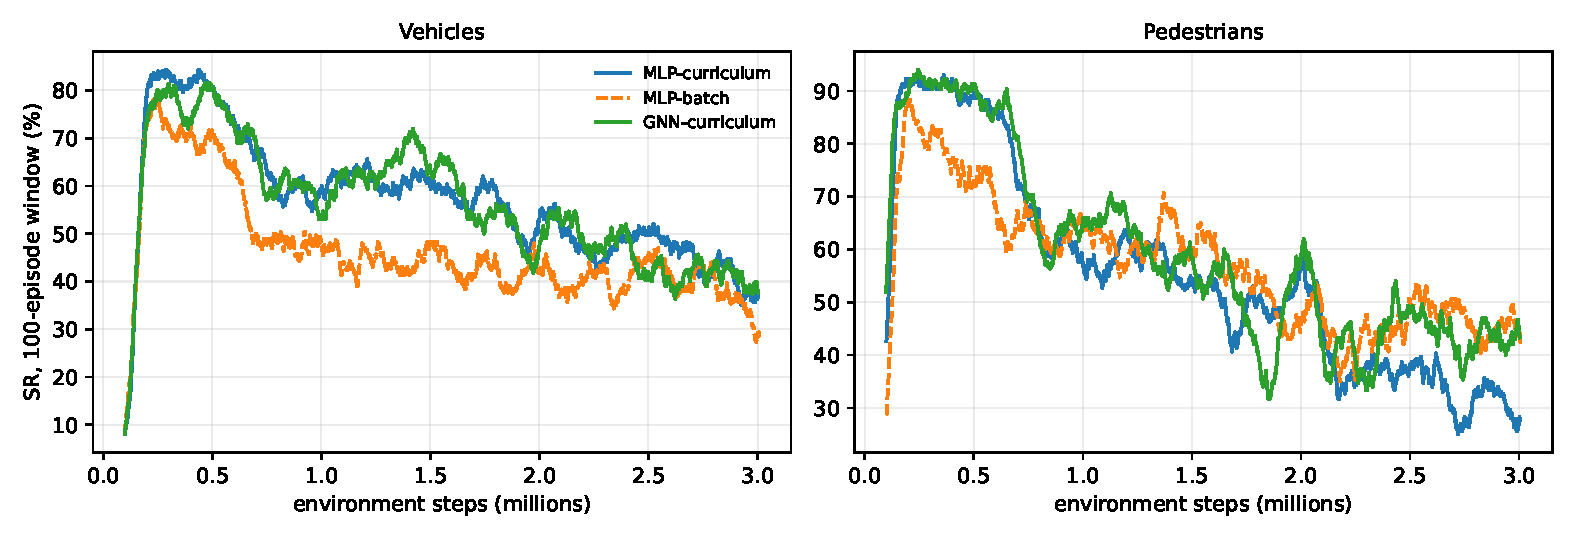
\includegraphics[width=\textwidth]{learning_curves}
  \caption{Tasso di successo a finestra (100 episodi) rispetto ai passi
  d'ambiente, tutte e quattro le celle.}
  \label{fig:curve}
\end{figure}

Una avvertenza va premessa alla \cref{fig:curve}: ogni curva è misurata
sul \emph{mix di livelli concorrente} della propria run --- gated per le
celle curriculum, uniforme per batch --- quindi i confronti verticali
tra bracci non sono omogenei finché il curriculum non ha sbloccato tutti
i livelli.

\paragraph{Fase iniziale: decollo indistinguibile.}
Tutte e quattro le celle salgono alla stessa velocità. L'SR veicoli a
finestra di 100 episodi supera per la prima volta il 30\% dopo
137--142K passi e il 50\% dopo 162--175K passi \emph{in ogni cella} ---
uno scarto sotto l'8\%, ben dentro il rumore. La parte notevole è
\emph{su che cosa} ciascuna policy ha superato quelle soglie: le celle
curriculum su esposizione solo-easy, le celle batch sul mix uniforme
completo, percorsi da \SI{100}{m} inclusi. A parità di budget, il
decollo iniziale non è stato il fattore discriminante tra i regimi.

\paragraph{Tempi di sblocco.}
Medium si è sbloccato praticamente nello stesso punto in entrambe le run
curriculum (al 26.1\% degli episodi in entrambe). Hard, invece, si è
sbloccato molto prima sotto il critic GNN: al 58.0\% dell'addestramento
contro il 71.0\% per MLP --- quest'ultimo coerente con lo scatto del cap
di pressione al 70\% del budget più che con il gate di competenza,
mentre la cella GNN ha raggiunto il gate hard \emph{per competenza}, e
ha quindi visto $\approx 40$\% episodi hard in più. Da $\approx 0.5$M
passi, infine, le curve batch si assestano sotto le due curve
curriculum, che si seguono da vicino; tutte derivano poi verso il basso
a fine addestramento (\cref{sec:dinamica}).

% ------------------------------------------------------------
\section{Prestazione finale}
\label{sec:prestazione}

\begin{table}[htbp]
  \centering\small
  \caption{I due strati di misura. Sopra: metriche cumulative di
  addestramento. Sotto: valutazione finale del checkpoint, 400 episodi
  per cella (401 per GNN-curriculum, \cref{sec:integrita}), l'unico
  confronto a distribuzione appaiata tra i bracci. Valori a livello di
  agente in \%; velocità in km/h (veicoli) e m/s (pedoni).}
  \label{tab:cumulative}
  \begin{tabular}{@{}lrrrrrrrr@{}}
    \toprule
    & \multicolumn{5}{c}{Veicoli} & \multicolumn{3}{c}{Pedoni} \\
    \cmidrule(lr){2-6}\cmidrule(l){7-9}
    Cella & SR & s$+$t & coll. & off. & vel. & SR & s$+$t & vel. \\
    \midrule
    MLP-curr.\ & 57.28 & 30.48 & 8.84 & 3.41 & 10.2 & 56.59 & 42.56 & 1.96 \\
    MLP-batch  & 46.31 & 23.61 & 17.33 & 12.76 & 18.7 & 57.06 & 42.03 & 1.61 \\
    GNN-curr.\ & 56.55 & 20.84 & 13.37 & 9.23 & 18.0 & 60.50 & 38.58 & 1.91 \\
    GNN-batch  & 49.41 & 22.75 & 17.56 & 10.28 & 26.6 & 58.03 & 41.11 & 1.45 \\
    \bottomrule
  \end{tabular}

  \vspace{1.2em}

  \begin{tabular}{@{}lrrrrrrrrr@{}}
    \toprule
    & \multicolumn{5}{c}{SR veicoli per scenario} &
      \multicolumn{3}{c}{Veicoli, compl.} & Ped. \\
    \cmidrule(lr){2-6}\cmidrule(lr){7-9}\cmidrule(l){10-10}
    Cella & easy & med. & hard & test & \textbf{tutti} & s$+$t & coll. & off. & SR \\
    \midrule
    MLP-curr.\ & 60.33 & 51.67 & 44.33 & 37.00 & \textbf{48.33} & 38.25 & 10.42 & 3.00 & 47.00 \\
    MLP-batch  & 41.33 & 31.00 & 29.00 & 18.00 & \textbf{29.83} & 31.17 & 26.00 & 13.00 & 48.92 \\
    GNN-curr.\ & 52.48 & 42.33 & 36.00 & 35.67 & \textbf{41.65} & 25.10 & 22.94 & 10.31 & 59.02 \\
    GNN-batch  & 55.67 & 42.00 & 33.33 & 25.67 & \textbf{39.17} & 23.83 & 26.92 & 10.08 & 48.67 \\
    \bottomrule
  \end{tabular}
  \\[0.3em]
  {\footnotesize Scenari easy/medium/hard su Town03, \emph{test} su Town05.}
\end{table}

\paragraph{Il contrasto primario, coppia MLP.}
Nella valutazione finale a distribuzione appaiata
(\cref{tab:cumulative}, pannello inferiore) la policy veicolo addestrata
a curriculum completa il 48.33\% dei percorsi contro il 29.83\% del
batch: $+18.5$ punti percentuali, con lo stesso segno in \emph{tutti e
quattro} gli scenari ($+19.0$, $+20.7$, $+15.3$, $+19.0$\,pp) e nel
cumulativo di addestramento ($+11.0$\,pp). Il margine è circa da due a
quattro volte la banda delle repliche a seed identico della
\cref{sec:gate}, e la sua coerenza tra scenari, livelli di difficoltà e
strati di misura è ciò che il design appaiato può offrire al posto della
replicazione dei seed.

\paragraph{Due modi diversi di fallire.}
I regimi producono guide riconoscibilmente diverse
(\cref{fig:fallimenti}). La policy batch è quasi due volte più veloce
(18.7 contro 10.2 km/h in addestramento) ma converte quella mobilità in
contatto: collisione 17.3\% contro 8.8\% e offroad 12.8\% contro 3.4\%
in addestramento, che si allargano a 26.0\% contro 10.4\% di collisione
in valutazione. La policy curriculum fallisce invece principalmente per
stallo (stuck$+$timeout 38.3\% contro 31.2\% in valutazione). Nessun
profilo domina l'altro su ogni asse --- il curriculum scambia velocità
per sicurezza --- ma sul criterio di successo rigoroso lo scambio si
risolve chiaramente a suo favore. I pedoni, per contro, sono
\emph{piatti} tra i bracci ovunque, entro $\pm 6$\,pp in ogni scenario:
il regime, in questa piattaforma, è una variabile della policy
\emph{veicolo}, e la struttura dei fallimenti pedonali è ripresa nella
\cref{sec:pedoni}.

\begin{figure}[t]
  \centering
  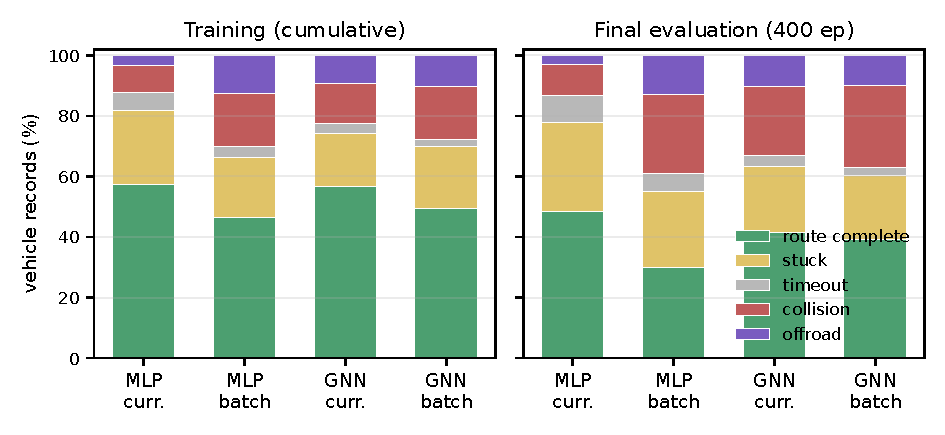
\includegraphics[width=\textwidth]{failure_modes}
  \caption{Composizione delle terminazioni dei veicoli per cella, in
  addestramento (cumulativo) e alla valutazione finale. Le due
  grammatiche del fallimento sono visibili a colpo d'occhio: dominata
  dallo stallo in MLP-curriculum, dominata dal contatto nelle celle
  batch, con le celle GNN in posizione intermedia.}
  \label{fig:fallimenti}
\end{figure}

\paragraph{Le celle GNN a colpo d'occhio.}
In addestramento la cella GNN-curriculum atterra entro il rumore di
MLP-curriculum sull'SR principale (56.55 contro 57.28\%) ma
ridistribuisce la massa dei fallimenti: meno stallo ($-9.6$\,pp), più
contatto e velocità molto più alta (18.0 contro 10.2 km/h) --- più
vicina alla mobilità delle celle batch, con il successo di una cella
curriculum. GNN-batch spinge le stesse tendenze oltre (26.6 km/h, la
cella più veloce) \emph{battendo} al contempo MLP-batch di $+3.1$\,pp in
addestramento e $+9.3$\,pp in valutazione: l'encoder del critic plasma
il profilo di rischio e interagisce con il regime
(\cref{sec:asse-arch}).

% ------------------------------------------------------------
\section{Dinamica entro la run}
\label{sec:dinamica}

Ogni curva della \cref{fig:curve} deriva verso il basso dopo il picco
iniziale. Per le celle curriculum questo è in parte meccanico --- il mix
concorrente si indurisce a ogni sblocco --- quindi la
\cref{tab:quartili} separa i due effetti: il pannello superiore riporta
le traiettorie per quartile complessive, quello inferiore la traiettoria
\emph{sui soli episodi easy}, dove il task è costante per costruzione.

\begin{table}[t]
  \centering\small
  \caption{SR veicoli per quartile di addestramento (\%). Sopra: tutti i
  livelli (confuso dal mix per le celle curriculum). Sotto: solo episodi
  easy, controllato per livello (easy resta $\approx 30$\% del mix dopo
  gli sblocchi). $\Delta$ = Q4 $-$ Q1.}
  \label{tab:quartili}
  \begin{tabular}{@{}lrrrrr@{}}
    \toprule
    Cella & Q1 & Q2 & Q3 & Q4 & $\Delta$ \\
    \midrule
    \multicolumn{6}{@{}l}{\emph{Tutti i livelli}} \\
    MLP-curr.\ & 68.9 & 61.1 & 54.4 & 44.7 & $-24.2$ \\
    MLP-batch  & 58.7 & 45.9 & 41.8 & 38.7 & $-20.0$ \\
    GNN-curr.\ & 66.6 & 62.2 & 54.5 & 42.9 & $-23.7$ \\
    GNN-batch  & 50.5 & 54.6 & 47.5 & 45.1 & $-5.4$ \\
    \midrule
    \multicolumn{6}{@{}l}{\emph{Solo livello easy}} \\
    MLP-curr.\ & 68.9 & 69.3 & 59.6 & 52.4 & $-16.5$ \\
    MLP-batch  & 64.2 & 52.0 & 48.9 & 45.6 & $-18.6$ \\
    GNN-curr.\ & 66.6 & 67.9 & 56.1 & 55.8 & $-10.8$ \\
    GNN-batch  & 59.7 & 62.8 & 54.3 & 53.3 & $-6.4$ \\
    \bottomrule
  \end{tabular}
\end{table}

\paragraph{Erosione, non solo indurimento del mix.}
Il pannello controllato per livello mostra che l'indurimento del mix
\emph{non} è tutta la storia: la prestazione a livello easy si erode
entro ogni run, da $-6.4$\,pp (GNN-batch, la cella più stabile) a
$-18.6$\,pp (MLP-batch). Le celle batch rendono il caso in modo pulito,
perché la loro distribuzione dei task è costante e il loro declino è
quindi interamente degradazione entro la run; i pedoni si erodono ancora
di più, fino a $-31.8$\,pp. Due meccanismi candidati sono compatibili
con i dati e non separabili a $n{=}1$: la co-adattazione tra classi,
poiché il comportamento dei pedoni degrada in parallelo e alimenta il
canale di hazard dei veicoli, e l'annealing dell'entropia --- che però
si completa solo dentro Q4, mentre l'erosione inizia già in Q3, e non
può quindi esserne l'unica causa. La conclusione pulita è
architetturale: sotto il critic GNN l'erosione è dimezzata o meglio,
qualunque ne sia il driver.

\paragraph{Due grammatiche del fallimento, un attrattore comune.}
La velocità media ordina le quattro celle --- 10.2 (MLP-curr.), 18.0
(GNN-curr.), 18.7 (MLP-batch), 26.6 km/h (GNN-batch) --- e i fallimenti
da contatto seguono lo stesso ordine, mentre lo stallo anti-correla. Ciò
che \emph{non} varia è la struttura interna dello stallo: in tutte e
quattro le celle le terminazioni stuck si decompongono quasi
identicamente e i passi medi di non-progresso coprono una banda stretta.
Regimi e critic cambiano \emph{quanto} una policy stalla, non
\emph{come} stalla. Coerentemente, il profilo lento-e-in-stallo
appartiene a esattamente una cella, MLP-curriculum: la sua gemella sotto
il critic GNN è quasi due volte più veloce con un terzo di stallo in
meno, allo stesso SR principale. L'equilibrio cauto documentato durante
lo sviluppo (\cref{sec:gate}) non è dunque una proprietà
dell'addestramento a curriculum in quanto tale, ma un bacino in cui la
run con critic MLP si è assestata e quella con critic GNN no: il regime
da solo non determina l'equilibrio.

% ------------------------------------------------------------
\section{Generalizzazione: da Town03 a Town05}
\label{sec:generalizzazione}

Lo scenario test colloca le stesse policy su Town05 --- layout a griglia
quadrata e più corsie, strutturalmente diverso da Town03 --- per 100
episodi con target di \SI{80}{m} e traffico come in addestramento.

\begin{figure}[t]
  \centering
  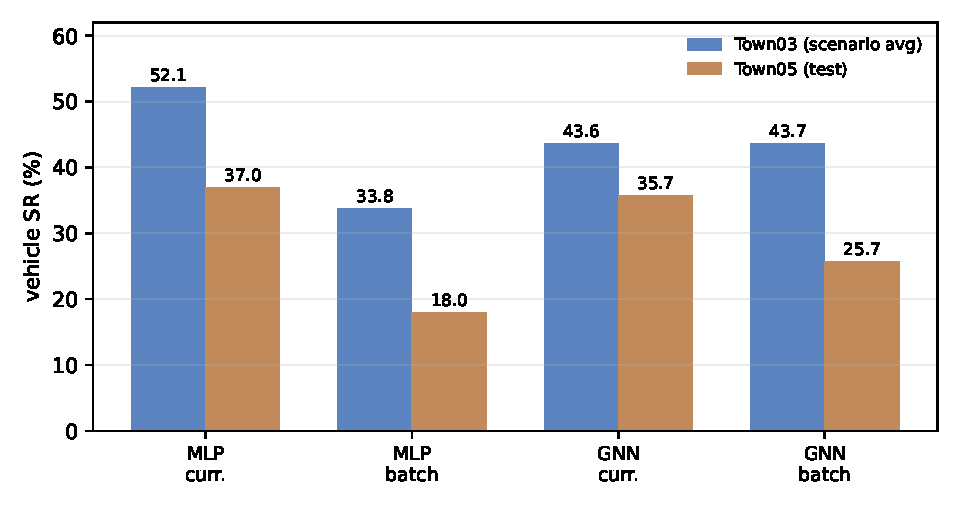
\includegraphics[width=0.70\textwidth]{town05_bars}
  \caption{SR veicoli: media degli scenari Town03 contro test Town05,
  per cella. Le celle curriculum calano meno; la coppia GNN è
  indistinguibile in-domain (43.6 contro 43.7\%) e si separa di 10\,pp
  sulla mappa mai vista.}
  \label{fig:town05}
\end{figure}

\paragraph{L'ordinamento sopravvive al cambio di mappa.}
Il curriculum completa il 37.0\% dei percorsi su Town05 contro il 18.0\%
del batch ($+19.0$\,pp): essenzialmente lo stesso margine in-domain. Il
calo assoluto dalla media degli scenari Town03 è quasi identico per i
due bracci ($-15.1$ contro $-15.8$\,pp), quindi il vantaggio del
curriculum non è un'idiosincrasia di Town03: si trasferisce per intero
su strade mai viste. Letta contro H2, la copertura iniziale più ampia
del regime batch non gli ha comprato \emph{alcun} vantaggio di
generalizzazione --- semmai il calo relativo è peggiore, dalla sua base
più bassa ($-47$\% contro $-29$\%). Ogni braccio, inoltre, fallisce su
Town05 nel modo in cui fallisce a casa, solo di più: la policy
curriculum stalla (stuck$+$timeout 50.7\%), la policy batch si schianta
(collisione 37.3\%).

\paragraph{Sotto il critic GNN il vantaggio esiste \emph{solo} fuori distribuzione.}
La coppia GNN affila il punto. In-domain i due bracci sono gemelli
statistici --- SR veicoli medio sugli scenari Town03 43.6\% (curriculum)
contro 43.7\% (batch) --- eppure su Town05 si separano di $+10.0$\,pp
(35.7 contro 25.7\%), con il calo più piccolo di ogni cella per
GNN-curriculum ($-7.9$\,pp) contro $-18.0$\,pp per GNN-batch. Dove la
coppia MLP mostrava un vantaggio del curriculum che \emph{si
trasferisce}, la coppia GNN ne mostra uno che \emph{compare} solo nel
trasferimento: evidenza con lo stesso segno, veicolata da due firme
diverse. I pedoni, infine, si trasferiscono con facilità --- $\approx
30$\,pp sopra i risultati hard di entrambi i bracci su Town03 ---
indicando ancora la fattibilità dei percorsi, non la generalizzazione
della policy, come loro collo di bottiglia (\cref{sec:pedoni}).

% ------------------------------------------------------------
\section{Asse architetturale: critic MLP contro GNN}
\label{sec:asse-arch}

L'asse secondario sostituisce solo l'encoder del critic; actor, reward,
ambiente e budget sono identici, quindi le differenze tra celle MLP e
GNN misurano come la \emph{stima del valore} plasma ciò che gli stessi
actor apprendono.

\begin{table}[t]
  \centering\small
  \caption{L'interazione architettura$\times$regime: SR veicoli
  curriculum-meno-batch (pp) per strato di misura, entro ciascuna
  architettura. Il delta di valutazione dei pedoni è aggiunto per
  completezza.}
  \label{tab:interazione}
  \begin{tabular}{@{}lrr@{}}
    \toprule
    $\Delta$(curr.\ $-$ batch) & Coppia MLP & Coppia GNN \\
    \midrule
    Cumulativo di addestramento (veic.) & $+10.97$ & $+7.14$ \\
    Valutazione complessiva (veic.) & $+18.50$ & $+2.48$ \\
    Valutazione, media Town03 (veic.) & $+18.33$ & $-0.06$ \\
    Valutazione, Town05 (veic.) & $+19.00$ & $+10.00$ \\
    Valutazione complessiva (ped.) & $-1.92$ & $+10.35$ \\
    \bottomrule
  \end{tabular}
\end{table}

\paragraph{L'effetto di regime dipende dal critic.}
La \cref{tab:interazione} condensa il risultato centrale della campagna.
Sotto il critic MLP il curriculum batte il batch con un margine ampio e
coerente tra gli strati; sotto il critic GNN lo stesso contrasto quasi
svanisce, con $+2.5$\,pp complessivi in valutazione --- dentro la banda
di rumore a seed identico --- ed esattamente zero in-domain. L'unica
componente del vantaggio del curriculum che \emph{si replica in entrambe
le architetture} è quella out-of-distribution: $+19.0$\,pp (MLP) e
$+10.0$\,pp (GNN) su Town05. H3 è quindi supportata nella sua forma
forte: l'encoder del critic cambia non solo l'entità, ma il \emph{luogo}
dell'effetto di regime.

\paragraph{Da dove viene l'interazione.}
La compressione è prodotta da due effetti architetturali asimmetrici,
uno per regime. Entro il batch il critic GNN \emph{aiuta}: $+3.1$\,pp in
addestramento e $+9.3$\,pp in valutazione rispetto a MLP-batch, con la
dinamica entro la run più stabile della campagna. È coerente con il
meccanismo che motiva i critic CTDE in primo luogo: sotto una
distribuzione mista con sei agenti interagenti, la stima strutturata del
valore dovrebbe aiutare di più dove il segnale è più rumoroso, cioè il
regime batch dal passo~0. Entro il curriculum, invece, il critic GNN
\emph{rimodella} più che migliorare: evita l'equilibrio difensivo,
sblocca hard per competenza anziché per cap di pressione, vede $\approx
40$\% episodi hard in più --- e converte tutto questo in mobilità e
contatto anziché in successo (SR $-6.7$\,pp rispetto a MLP-curriculum).
I pedoni mostrano l'interazione speculare: il critic GNN li solleva
sotto curriculum ($+12.0$\,pp in valutazione, la miglior cella pedoni
della campagna al 59.0\%) ma non sotto batch.

Il pattern è internamente coerente su quattro strati di misura ed
entrambe le classi di agenti, ma le sue grandezze portano la consueta
qualifica $n{=}1$ (\cref{sec:minacce}): il delta complessivo di
$+2.5$\,pp della coppia GNN esplicitamente \emph{non} è rivendicato come
vantaggio del curriculum, e il risultato rivendicato è il suo contrasto
con la coppia MLP più la componente Town05 replicata tra le
architetture.

% ------------------------------------------------------------
\section{Limiti strutturali dei pedoni}
\label{sec:pedoni}

I risultati dei pedoni vanno letti contro un vincolo che nessun regime
di addestramento può rimuovere: la topologia dei marciapiedi di Town03
spesso non può fornire il task nominale. Le diagnostiche di generazione
dei percorsi pedonali sono infatti statisticamente indistinguibili tra
le quattro celle --- percorsi under-target 55.1--55.9\% dei record, flag
too-short 7.9--9.2\%, percorsi da respawn 13.4--14.1\% --- e questa
\emph{invarianza} è il punto: sono proprietà della mappa e del planner,
non delle policy, e fissano quindi un soffitto comune a ogni cella.

L'SR pedoni cala poi monotonicamente con il livello in ogni cella (in
addestramento easy 70--83\%, medium 53--60\%, hard 29--44\%) e la
valutazione a distribuzione appaiata riproduce il gradiente. Un collasso
che sopravvive a due architetture, due regimi e due strati di misura
mentre le diagnostiche restano costanti è guidato dalla geometria del
task, e il controfattuale Town05 rende concreta l'attribuzione: con
target di \SI{80}{m} l'SR pedoni balza a 54--71\% in ogni cella, da 15 a
31\,pp \emph{sopra} il risultato hard su Town03 e per giunta su una
mappa mai vista --- se il collasso fosse un limite di policy, strade
nuove dovrebbero nuocere, non aiutare. Entro l'inviluppo di fattibilità
le differenze di policy restano comunque visibili, e una cella si separa
dal gruppo in valutazione (GNN-curriculum, 59.0\% contro 47--49\%
altrove). La conseguenza metodologica resta però vincolante: i tassi di
successo medium e hard dei pedoni non sono una misura pulita della
qualità della policy, quindi la tesi confronta i pedoni solo entro
livello e tra bracci.

% ------------------------------------------------------------
\section{Verdetti sulle ipotesi}
\label{sec:verdetti}

\begin{table}[t]
  \centering\small
  \caption{Ipotesi contro evidenza (contrasti appaiati, $n{=}1$ per
  cella; delta in pp di SR veicoli salvo diversa indicazione).}
  \label{tab:ipotesi}
  \begin{tabular}{@{}p{2.0cm}p{4.3cm}p{2.3cm}p{4.2cm}@{}}
    \toprule
    Ipotesi & Predizione & Verdetto & Evidenza \\
    \midrule
    H1 (curriculum) & migliore efficienza campionaria \emph{iniziale} & rigettata &
      decollo identico nelle quattro celle (50\% a 162--175K passi) \\
    & prestazione finale più alta & supportata sotto MLP, non sotto GNN
      in-domain & $+18.5$ (MLP) contro $+2.5$ (GNN) in valutazione \\
    & rischio di plateau od oblio su hard & rimodellato &
      erosione tardiva reale ma \emph{di piattaforma}: $\Delta$Q1$\to$Q4
      per livello da $-6$ a $-19$\,pp \\
    \addlinespace
    H2 (batch) & piena copertura dal passo 0 & confermata (meccanica) &
      tutti i livelli entro i primi 20 episodi \\
    & segnale iniziale più rumoroso & non visibile &
      stesso decollo, sul mix più difficile \\
    & copertura $\to$ robustezza su mappa nuova & rigettata &
      calo su Town05 uguale o peggiore in entrambe le coppie
      ($-15.8$/$-18.0$ contro $-15.1$/$-7.9$\,pp) \\
    \addlinespace
    H3 (interazione) & l'effetto di regime può dipendere dall'encoder
      del critic & supportata (forma forte) &
      effetto in-domain $+18.3$ (MLP) contro $-0.1$ (GNN); solo la
      componente Town05 si replica \\
    \bottomrule
  \end{tabular}
\end{table}

Due cose sopravvivono a ogni cella, ogni strato ed entrambe le
architetture: il vantaggio del curriculum sulla mappa mai vista, e il
ruolo del regime come variabile della policy \emph{veicolo} che rimodella
la composizione dei fallimenti. Ciò che non è sopravvissuto è
l'aspettativa popolare da entrambi i lati: il curriculum non ha appreso
più in fretta all'inizio, e la copertura più ampia del batch non ha
comprato robustezza.

% ------------------------------------------------------------
\section{Discussione}
\label{sec:discussione}

\paragraph{Non la velocità di apprendimento, ma la selezione dell'equilibrio.}
L'asse su cui i curricula sono classicamente attesi ripagare non ha
mostrato nulla. Una lettura plausibile è che il design della reward di
questa piattaforma risolva già il problema per cui i curricula vengono
di solito ingaggiati: con bonus densi per waypoint e shaping sulla
distanza (\cref{sec:reward}), anche i percorsi da \SI{100}{m}
forniscono segnale di apprendimento fin dai primi episodi, quindi i task
facili non servono per l'avvio. È una \emph{condizione di scope} su H1,
più che una confutazione del curriculum learning in generale. Ciò che
l'ordinamento ha cambiato è \emph{quale policy lo stesso apprendista è
diventato}, e la meccanica è visibile nei vincoli: completare un
percorso da \SI{100}{m} entro l'orizzonte di mille passi richiede una
velocità media sana, quindi una policy esposta ai percorsi hard dal
passo~0 deve guidare veloce per riuscire del tutto --- e paga in
collisioni --- mentre una policy che spende il suo primo quarto di
addestramento su percorsi da \SI{30}{m} può riuscire lentamente, e
cementa la cautela. L'ordinamento agisce dunque da \emph{selettore di
equilibri} sul trade-off velocità--sicurezza più che da acceleratore, e
le celle GNN sostengono la lettura dall'altro lato: con uno stimatore di
valore diverso lo stesso curriculum ha selezionato un equilibrio più
veloce. Va infine osservato che l'erosione entro la run è di piattaforma
e che l'ordinamento non la causa né la previene: i numeri cumulativi
\emph{finali} sottostimano i picchi di metà addestramento in ogni
configurazione, e la selezione del checkpoint cambierebbe le
conclusioni.

\paragraph{Generalizzazione: il beneficio portabile.}
L'unico vantaggio replicato in entrambe le architetture è il margine su
Town05, ottenuto \emph{nonostante} la copertura in-domain più ampia del
batch. Un meccanismo provvisorio è coerente con entrambe le coppie: la
policy batch si co-adatta per l'intero budget a una singola
distribuzione stazionaria, mentre la policy curriculum deve restare
competente attraverso una sequenza \emph{mutevole} di distribuzioni ---
una forma blanda di regolarizzazione implicita per non-stazionarietà. A
$n{=}1$ per cella questa resta un'ipotesi; ciò che i dati stabiliscono è
la direzione e la sua replicazione tra architetture.

\paragraph{La copertura parallela dei task rivisitata.}
La cornice a mondo condiviso è stata adottata per il throughput, con
campioni correlati e non-stazionarietà reciproca accettati come costi;
col senno di poi la campagna mostra quei ``costi'' fare lavoro
scientifico di prim'ordine. L'equilibrio difensivo esiste \emph{solo}
perché le reward dei veicoli sono condizionate a un canale di hazard
alimentato dal comportamento dei pedoni, e il risultato architetturale
punta nella stessa direzione: sostituire un critic piatto con uno che
modella gli agenti come nodi interagenti ha cambiato gli esiti in ogni
cella, cosa impossibile se la struttura tra agenti fosse trascurabile.
In assenza di un controllo a un agente per mondo, però, il beneficio di
throughput resta un argomento di design e non una misura.

% ------------------------------------------------------------
\section{Minacce alla validità e limiti di scope}
\label{sec:minacce}

\paragraph{Non-determinismo del simulatore e dimensione campionaria.}
La minaccia dominante è quantificata anziché assunta: tre run a
lunghezza piena con codice, configurazione e seed byte-identici hanno
prodotto tassi di successo cumulativi dei veicoli tra 52.2 e 62.4\%
(\cref{sec:gate}). Ogni effetto è letto contro questa banda di
$\sim$10\,pp, e le differenze al suo interno non sono mai attribuite a
un fattore sperimentale. A ciò si somma il fatto che ogni cella contiene
una sola run (\cref{sec:campagna}): l'appaiamento dei seed rende i
contrasti internamente puliti, e il contrasto primario porta con sé una
replicazione incorporata perché è osservato sotto entrambe le
architetture, ma nessuna inferenza statistica formale è possibile a
questo $n$, e nessuna è rivendicata.

\paragraph{Rumore di valutazione, reward e mappe.}
In valutazione, 100 episodi per scenario significano 300 record
veicolo: a tassi di fascia media il solo errore standard binomiale è
$\approx$3\,pp per scenario, quindi le differenze di pochi punti a
livello di singolo scenario non sono individualmente significative e si
interpretano solo i pattern tra scenari. La funzione di reward, inoltre,
è stata calibrata attraverso iterazioni eseguite per lo più su
configurazioni bloccate su easy, quindi lo shaping del trunk può essere
implicitamente sbilanciato verso i percorsi corti; entrambi i regimi
condividono però la reward identica, quindi il contrasto primario resta
internamente valido e l'avvertenza riguarda la sola prestazione
\emph{assoluta} sui percorsi hard. La generalizzazione, infine, è
misurata su esattamente un trasferimento, e le affermazioni sono
limitate a questa coppia di mappe. Va anche ricordato che la pipeline di
valutazione stessa ha fallito la validità una volta e che il difetto di
lunghezza dei percorsi ha ridefinito silenziosamente la distribuzione
dei task per un'intera era di esperimenti (\cref{sec:validita}): in una
piattaforma custom, gli effetti apparenti devono prima sopravvivere alla
domanda ``lo strumento sta misurando ciò che dichiara?''.

\paragraph{Limiti di scope.}
Il design fissa infine diverse dimensioni, e i risultati non vanno letti
oltre di esse (\cref{sec:campagna}). L'architettura degli \emph{actor} è
fissa, quindi l'asse GNN parla della sola stima del valore sotto CTDE; la
cornice a mondo condiviso non è ablata, quindi il suo contributo causale
è caratterizzato e non isolato; le osservazioni sono privilegiate e non
percettive, quindi nulla segue per pipeline basate su camera o lidar; e
l'algoritmo e la versione della piattaforma sono unici, quindi altri
algoritmi possono interagire diversamente con l'ordinamento.


% Blocco III — Possibili evoluzioni
% ============================================================
% v2 — Capitolo 5: Possibili evoluzioni
% Blocco III di IV. Budget: ~2 pagine.
% Le sette direzioni della v1 (§7.2), riorganizzate in tre gruppi
% per prossimità al lavoro svolto anziché in lista piatta.
% ============================================================
\chapter{Possibili evoluzioni}
\label{ch:evoluzioni}

Le direzioni che seguono sono ordinate per prossimità: prima quelle che
consolidano l'evidenza già raccolta, poi quelle che rimuovono i limiti
noti della piattaforma, infine quelle che estendono la domanda a un
terreno nuovo. Le prime due categorie sono realizzabili sul codice
esistente e su un budget di calcolo confrontabile con quello di questa
tesi, la terza no.

\section{Consolidare l'evidenza}
\label{sec:evo-evidenza}

\paragraph{Replicazione dei seed.}
È l'estensione più diretta e la più importante. Il design è stato
tagliato da tre seed appaiati per cella a uno per ragioni di calcolo
(\cref{sec:campagna}), e questa riduzione è la fonte principale di
cautela in tutta la tesi. Rieseguire la matrice $2\times2$ a $n{=}3$
trasformerebbe i casi di studio appaiati in stime di distribuzione e
metterebbe alla prova direttamente l'entità dell'interazione
architettura$\times$regime, che è oggi il risultato più forte e al tempo
stesso il meno replicato. Il costo è noto e lineare: otto run da tre
milioni di passi in aggiunta alle quattro esistenti.

\paragraph{Spiegare l'erosione.}
La degradazione entro la run controllata per livello
(\cref{tab:quartili}) è presente in tutte le celle e dimezzata sotto il
critic relazionale, e la tesi ne identifica due cause candidate senza
poterle separare. Due ablazioni mirate lo farebbero: congelare una
classe di agenti a metà addestramento isolerebbe la co-adattazione tra
classi, e spostare l'ancora dell'annealing di entropia isolerebbe lo
schedule di esplorazione. Entrambe sono modifiche di poche righe sulla
piattaforma esistente e girano al budget diagnostico del protocollo di
gate.

\paragraph{Selezione del checkpoint.}
Poiché i numeri finali sottostimano i picchi di metà addestramento in
ogni cella (\cref{sec:discussione}), un'analisi che valuti il
\emph{miglior} checkpoint anziché l'ultimo direbbe se l'ordinamento dei
task cambi anche il punto in cui la competenza culmina, e non solo
quello in cui atterra. I checkpoint intermedi sono già su disco: è
un'estensione della sola pipeline di valutazione.

\section{Rimuovere i limiti della piattaforma}
\label{sec:evo-piattaforma}

\paragraph{Generazione dei percorsi pedonali.}
Con più della metà dei percorsi pedonali sotto target su Town03
(\cref{sec:pedoni}), un planner consapevole della fattibilità ---
esplorazione più profonda delle ramificazioni, target adattivi per
regione di spawn, rinuncia esplicita quando la topologia locale non
sostiene la distanza richiesta --- è la correzione d'ambiente a maggior
leva: renderebbe interpretabili i tassi di successo medium e hard che
questa tesi è costretta a leggere solo entro livello, oggi vincolati da
un soffitto comune a tutte le celle.

\paragraph{Co-design di reward e curriculum.}
Il tuning della reward guidato da gate è girato per lo più su
configurazioni bloccate su easy (\cref{sec:minacce}), quindi lo shaping
del trunk può essere implicitamente sbilanciato verso i percorsi corti.
Ricalibrare i termini chiave sul mix completo quantificherebbe quanto
dell'effetto di regime sia mediato dalla calibrazione della reward, e
metterebbe alla prova la spiegazione avanzata per il fallimento di H1.

\section{Estendere la domanda}
\label{sec:evo-estensioni}

\paragraph{Estensioni architetturali sul critic.}
L'infrastruttura espone già encoder basati su attenzione (GAT) e la
normalizzazione del valore PopArt dietro flag di configurazione
(\cref{sec:critic}). Vista la forza dell'interazione osservata con
l'encoder del critic, queste non sono aggiunte esotiche ma le celle
successive naturali della stessa matrice: se sostituire un MLP con un
message passing a media sposta il \emph{luogo} dell'effetto di regime,
la domanda immediatamente successiva è se un'aggregazione pesata da
attenzione lo sposti ancora.

\paragraph{Curricula adattivi.}
Il gate di competenza di questa tesi è un sequenziatore fisso a due
soglie. Curricula che adattano le quote di livello in continuo --- per
esempio campionando in proporzione al progresso di apprendimento
misurato per livello --- metterebbero alla prova se l'effetto di
selezione dell'equilibrio sopravviva a un ordinamento a grana molto più
fine, o se dipenda proprio dalla discontinuità degli sblocchi.

\paragraph{Scalare la cornice.}
La copertura parallela dei task è stata fissata a $3{+}3$ agenti.
Scalare il mondo condiviso verso decine di agenti --- dove la struttura
relazionale del critic GNN dovrebbe contare di più --- trasforma la
cornice di coesistenza stessa in una variabile sperimentale, e sposta il
lavoro dalla caratterizzazione di un effetto alla sua legge di scala. È
l'unica direzione che richiede un'infrastruttura di calcolo
sostanzialmente diversa da quella usata qui
(\cref{app:riproducibilita}).


% Blocco IV — Conclusioni
% ============================================================
% v2 — Capitolo 6: Conclusioni
% Blocco IV di IV. Budget: ~2 pagine.
% ============================================================
\chapter{Conclusioni}
\label{ch:conclusioni}

Questa tesi ha chiesto se ordinare i task di addestramento dal facile al
difficile produca un comportamento di guida multi-agente misurabilmente
diverso rispetto al presentare tutte le difficoltà insieme, a parità di
budget, in un ambiente CARLA a mondo condiviso addestrato con MAPPO. La
risposta è sì --- ma non lungo l'asse su cui i curricula vengono di
solito proposti.

\paragraph{L'ordinamento non ha accelerato l'apprendimento.}
Tutte e quattro le celle della campagna hanno raggiunto le stesse soglie
iniziali di competenza agli stessi conteggi di passi, con uno scarto
sotto l'8\% (\cref{sec:efficienza}), e questo pur avendole superate su
mix di difficoltà completamente diversi. La spiegazione più plausibile è
che il reward shaping denso di questa piattaforma fornisca già segnale
di apprendimento anche sui task difficili, rendendo superfluo l'avvio
graduale: una condizione di scope su H1, non una confutazione del
curriculum learning in generale.

\paragraph{L'ordinamento ha selezionato ciò che la policy è diventata.}
Sotto il critic MLP il curriculum ha prodotto un guidatore cauto e
incline allo stallo e il batch uno veloce e incline alle collisioni; sul
criterio di successo rigoroso lo scambio si è risolto a favore del
curriculum di $+18.5$\,pp in valutazione, coerentemente in tutti e
quattro gli scenari (\cref{sec:prestazione}). L'ordinamento dei task
agisce cioè da \emph{selettore di equilibri} sul trade-off
velocità--sicurezza, più che da acceleratore.

\paragraph{L'effetto è condizionato dalla stima del valore.}
Sotto un critic GNN l'effetto di regime in-domain è svanito
($-0.1$\,pp) mentre l'architettura ha recuperato la cella batch e
rimodellato la cella curriculum: una forte interazione
architettura$\times$regime (\cref{sec:asse-arch}). Il regime di
addestramento non è quindi una leva indipendente dal resto dello stack,
e riportarne l'effetto senza dichiarare l'architettura del critic è
riportarne solo metà.

\paragraph{Il beneficio portabile è la generalizzazione.}
L'unica componente del vantaggio del curriculum replicata in entrambe le
architetture è il margine su una città mai vista in addestramento
($+19.0$ e $+10.0$\,pp su Town05), ottenuta contro l'intuizione
copertura-implica-robustezza che motivava H2
(\cref{sec:generalizzazione}). È il risultato che questa tesi difende
con più forza, perché è l'unico osservato due volte in modo
indipendente.

\paragraph{Specificità di classe e limiti della piattaforma.}
I pedoni sono risultati in larga parte insensibili al regime, vincolati
dalla fattibilità dei percorsi più che dalla qualità della policy
(\cref{sec:pedoni}); e ogni cella ha mostrato erosione tardiva entro la
run a livello di task fissato, indipendente dal regime
(\cref{sec:dinamica}). Le scelte di regime calibrate sulla classe forte
non vanno assunte trasferibili alla debole.

\bigskip

Oltre ai risultati, la tesi contribuisce l'apparato che li ha resi
misurabili: un framework di confronto a parità di budget con
configurazioni appaiate per seed e byte-identiche; un protocollo di
sviluppo guidato da gate con un registro esplicito di modifiche
promosse, rigettate e consapevolmente mantenute; un resoconto
documentato di come i difetti di validità dell'ambiente possano
mascherarsi da effetti di policy, con le loro firme di rilevamento; e un
metro di varianza da repliche a seed identico contro cui ogni
affermazione viene letta. In un contesto in cui un singolo bug del
simulatore ha spostato la metrica principale di cinquanta punti
percentuali senza che nulla cambiasse nella policy, questa disciplina di
misura --- e non un singolo numero --- è ciò che rende il confronto
significativo.

Resta il limite che la tesi dichiara apertamente e che il
\cref{ch:evoluzioni} mette in cima all'elenco: con una run per cella,
ogni contrasto è un caso di studio appaiato letto contro una banda di
rumore, non la stima di una distribuzione. La replicazione sui seed
della matrice $2\times2$ è il passo che trasformerebbe le conclusioni
qui riportate da direzioni ben corroborate in effetti quantificati.


% ----------------- Appendici (fuori conteggio) ---------------
\appendix
% ============================================================
% v2 — Appendici A–B (snelle, fuori conteggio pagine)
% A: iperparametri e configurazione (tabellati anziché dump YAML)
% B: riproducibilità
% Valori verificati dagli snapshot in latex/configs/ (2026-07-14).
% ============================================================

\chapter{Osservazioni e reward per componente}
\label{app:obs-reward}

Le due tabelle che seguono danno il dettaglio per componente degli spazi
di osservazione (\cref{sec:osservazioni}) e della funzione di reward
(\cref{sec:reward}), la cui struttura e il cui razionale sono descritti
nel \cref{ch:piattaforma}. Tutti i valori sono verificati dal codice del
trunk di campagna.

\begin{table}[h]
  \centering\small
  \caption{Layout delle osservazioni. Le barre indicano costanti di
  normalizzazione; le feature dei vicini sono nel sistema di riferimento
  dell'ego. TTC $=$ time-to-collision.}
  \label{tab:obs}
  \begin{tabular}{@{}llp{8.0cm}@{}}
    \toprule
    Dim. & Gruppo & Contenuto \\
    \midrule
    \multicolumn{3}{@{}l}{\emph{Veicolo (47D)}} \\
    0--12  & Ego e percorso   & velocità (/30), accelerazione (/10), modulo (/120 km/h), heading; distanza (/\SI{50}{m}) e bearing al waypoint successivo; offset laterale in corsia; progresso continuo \\
    13--23 & Semaforo, vicini & flag e stato del semaforo; 3 veicoli più prossimi entro \SI{50}{m} (offset long.\ e lat.\ /50, velocità relativa /30) \\
    24--33 & Anteprima e geometria & sterzo precedente; waypoint $+1/+3/+5$; errore di heading; angolo curva imminente; errore laterale con segno \\
    34--43 & Pedoni e hazard  & 2 pedoni più prossimi, stesse 3 feature; rischio TTC e occupazione del corridoio, vs.\ veicoli e vs.\ pedoni \\
    44--46 & Progresso/tempo  & passi senza progresso (/300); flag anti-loop; tempo rimanente \\
    \midrule
    \multicolumn{3}{@{}l}{\emph{Pedone (26D)}} \\
    0--11  & Ego e waypoint   & posizione ($x,y$ /500, $z$ /50); velocità (/5); vettore frontale; distanza (/\SI{100}{m}) e bearing al waypoint; flag marciapiede \\
    12--17 & Veicoli vicini   & 2 più prossimi entro \SI{50}{m}: stesse 3 feature \\
    18--25 & Percorso e hazard & completamento; waypoint $+1/+3$ (/100); errore di heading; rischio TTC e occupazione vs.\ veicoli \\
    \bottomrule
  \end{tabular}
\end{table}

\begin{table}[h]
  \centering\small
  \caption{Componenti della reward. Le righe veicolo ``gated'' sono
  sospese durante l'attesa a un semaforo rosso/giallo; le righe marcate
  $^{\dagger}$ richiedono inoltre $\mathit{safe\_to\_push}$
  ($\mathit{hazard} < 0.85$) e allineamento al percorso $> 0.25$.}
  \label{tab:reward}
  \begin{tabular}{@{}p{3.2cm}p{5.2cm}p{4.4cm}@{}}
    \toprule
    Componente & Trigger & Valore \\
    \midrule
    \multicolumn{3}{@{}l}{\emph{Veicolo}} \\
    Waypoint raggiunto / saltato & per waypoint avanzato / saltato & $+100$ / $-10$ \\
    Progresso denso       & variazione della distanza dal waypoint & $+4.0$ per metro guadagnato \\
    Collisione            & primo contatto (terminale) & $-500$ \\
    Fuori corsia / eccesso di velocità & $>$ \SI{2}{m} dal centro corsia \ / \ $v > 50$ km/h & $-0.5$ per metro \ / \ $-0.10$ per km/h \\
    Inattività (gated)    & velocità $< 2.5$ km/h & $-0.15$ \\
    Bonus di partenza (gated$^{\dagger}$) & acceleratore da fermo & $(0.20 + 0.30\,u)\cdot\text{thr}\cdot\text{align}$, freno simmetrico; $u = \min(\text{no-progress}/200, 1)$ \\
    Shaping velocità minima (gated$^{\dagger}$) & velocità sotto / sopra 8 km/h & $-0.04\,(8 - v)\cdot\text{align}$ / $+0.15\cdot\text{align}$ \\
    Rampa di non-progresso (gated) & $>$ 100 passi senza waypoint & $-0.004$ per passo, tetto $-1.0$ \\
    Sterzo fluido / a strattoni & $|\Delta \text{steer}| < 0.1$ a $> 5$ km/h \ / \ $> 0.5$ & $+0.1$ / $-0.3$ \\
    Anti-loop             & rilevatore di loop attivo & $-1.0$ \\
    \midrule
    \multicolumn{3}{@{}l}{\emph{Pedone}} \\
    Waypoint raggiunto / saltato & per waypoint avanzato / saltato & $+50$ / $-10$ \\
    Progresso denso       & variazione della distanza dal waypoint & $+2.0$ per metro guadagnato \\
    Collisione            & primo contatto (terminale) & $-50$ \\
    Marciapiede / carreggiata & per passo su marciapiede / corsia & $+0.2$ / $-0.3$ \\
    Passo di camminata    & velocità $\in [1.2, 2.6]$ m/s & $+0.3$ \\
    Inattività / corsa    & velocità $< 0.15$ m/s \ / \ $> 3.0$ m/s & $-0.15$ / $-0.7$ per m/s oltre \\
    Anti-loop             & rilevatore di loop attivo & $-1.0$ \\
    \bottomrule
  \end{tabular}
\end{table}

\chapter{Registro condensato degli esperimenti}
\label{app:registro}

La \cref{tab:candidati} elenca i candidati valutati durante la fase di
sviluppo guidata da gate (\cref{sec:gate}) con il verdetto e l'esito di
sintesi. Le run A/B sono da $3\times10^{5}$ passi, seed 999, bloccate su
easy salvo diversa indicazione; i delta sono rispetto alla baseline
appaiata della loro era e \emph{non} sono confrontabili tra versioni
dell'ambiente (\cref{sec:validita}). Il registro completo, con
meccanismi e identificatori di run per candidato, è mantenuto nel
repository.

\begin{table}[!htbp]
  \centering\small
  \caption{Registro condensato dei candidati.}
  \label{tab:candidati}
  \begin{tabular}{@{}L{4.5cm}L{2.6cm}L{2.6cm}L{4.3cm}@{}}
    \toprule
    Candidato & Tipo & Verdetto & Sintesi \\
    \midrule
    Correzione lunghezza percorsi & bug fix & adottato & $\approx +50$\,pp SR (cambio di distribuzione) \\
    Correzione seed percorsi & bug fix & adottato & ripristina l'appaiamento A/B \\
    Osservabilità 47D & osservazione & adottato & baseline sana, var.\ spiegata 0.983 \\
    Blocco di reward shaping anti-stallo & reward & promosso & nucleo della \cref{sec:reward} \\
    Rimozione guardia di progresso & reward & promosso & SR $+4.7$\,pp, s$+$t $-3.5$\,pp \\
    Tolleranza hazard $0.75 \to 0.85$ & reward & promosso & 5/5: SR $+2.3$\,pp, s$+$t $-3.0$\,pp \\
    Tetto attraversamenti $8 \to 3$ & percorsi & promosso & SR $+9.2$\,pp, coll.\ $-2.3$\,pp, off.\ $-2.2$\,pp \\
    Schedule di entropia a frazione & ottimizzatore & promosso & meccanismo stabile, nessuna instabilità \\
    Riparazione value loss & ottimizzatore & mantenuto (gate fallito) & var.\ spiegata $0 \to 0.87$; collisione $+3.3$\,pp \\
    Sconto $0.99 \to 0.997$ & ottimizzatore & mantenuto (falsificato) & timeout $\to$ collisione $\approx$ 1:1 \\
    Penalità di collisione $\times 10$ & reward & mantenuto (falsificato) & collisione piatta: limite di percezione, non di peso \\
    Terminazione precoce da stuck & dinamica env & rigettato & SR $-2.9$\,pp, s$+$t $+7.1$\,pp \\
    Retuning banda di passo pedoni & reward & rigettato & overshoot peggiore; declino in Q4 \\
    \texttt{route\_short} come successo & misura & revertito & violava il criterio di successo \\
    \bottomrule
  \end{tabular}
\end{table}

\chapter{Configurazione e iperparametri}
\label{app:config}

La \cref{tab:iperparametri} riporta la configurazione completa delle
quattro run di campagna. Tutti i valori sono identici tra le celle a
meno dei due flag sperimentali (\texttt{mode} e \texttt{use\_gnn}),
proprietà verificata con un diff diretto dei \texttt{run\_config.json}
scritti al lancio, che restano il riferimento autoritativo per ogni
singola run. Le famiglie di livelli per densità di traffico e miste sono
definite in configurazione ma inutilizzate in questa tesi
(\cref{sec:campagna}).

\begin{table}[!htbp]
  \centering\small
  \setlength{\tabcolsep}{4pt}
  \caption{Configurazione delle run di campagna.}
  \label{tab:iperparametri}
  \begin{tabular}{@{}llL{9.0cm}@{}}
    \toprule
    Gruppo & Parametro & Valore \\
    \midrule
    \multicolumn{3}{@{}l}{\emph{Ottimizzazione (PPO/MAPPO)}} \\
    & learning rate & $5\times10^{-4}$ \\
    & $\gamma$ & 0.997 \\
    & GAE $\lambda$ & 0.95 \\
    & clip PPO $\varepsilon$ & 0.2 \\
    & penalità KL & attiva; target 0.02, coefficiente iniziale 0.3 \\
    & gradient clipping & 0.5 \\
    & \texttt{vf\_clip\_param} & $10^{6}$ (clamp non vincolante) \\
    & \texttt{vf\_loss\_coeff} & 0.05 \\
    & coefficiente di entropia & schedule a frazione del budget: $0.03$ a $0.0$, $0.005$ a $0.83$ \\
    \addlinespace
    \multicolumn{3}{@{}l}{\emph{Rollout e batching}} \\
    & frammento di rollout & 200 passi \\
    & batch di addestramento & 8{.}000 passi \\
    & minibatch SGD & 256 \\
    & epoche SGD per batch & 15 \\
    & budget totale & $3\times10^{6}$ passi d'ambiente \\
    & frequenza di checkpoint & ogni $10^{5}$ passi \\
    \addlinespace
    \multicolumn{3}{@{}l}{\emph{Modello}} \\
    & actor (entrambe le classi) & MLP, 2 strati nascosti da 256 \\
    & critic MLP & $225 \to 256 \to 256 \to 1$ \\
    & critic GNN & embedding di nodo 64, 2 layer di message passing, aggregazione a media, ELU \\
    & PopArt, attenzione & disabilitati \\
    \addlinespace
    \multicolumn{3}{@{}l}{\emph{Curriculum}} \\
    & finestra di competenza & 50 episodi (deve essere piena) \\
    & metrica di sblocco & minimo dell'SR a finestra sulle due policy \\
    & soglia medium / hard & 0.70 / 0.60 \\
    & quota minima di budget & easy $\geq 0.20$ prima di medium; medium $\geq 0.28$ prima di hard \\
    & cap di pressione & medium al 30\% del budget, hard al 70\% \\
    & pesi di campionamento & $1.00 / 1.17 / 1.17$ ($\to 0.30/0.35/0.35$) \\
    & vincoli di budget & easy $\leq 0.30$, medium $\leq 0.35$, hard $\geq 0.35$ \\
    & probation & 2 blocchi dopo lo sblocco (1 dopo un cap); peso hard $0.85$ \\
    \addlinespace
    \multicolumn{3}{@{}l}{\emph{Batch}} \\
    & campionamento & mescolamento stratificato senza reinserimento, finestra 3 \\
    \addlinespace
    \multicolumn{3}{@{}l}{\emph{Livelli (difficoltà = lunghezza percorso)}} \\
    & easy / medium / hard & Town03, \SI{30}{m} / \SI{60}{m} / \SI{100}{m} \\
    & test (solo valutazione) & Town05, \SI{80}{m} \\
    & traffico NPC & 15 veicoli, 30 pedoni in ogni livello \\
    \bottomrule
  \end{tabular}
\end{table}

\chapter{Riproducibilità}
\label{app:riproducibilita}

\paragraph{Stack software.}
CARLA 0.9.16 (server e API Python); Python 3.11.9; PyTorch 2.7
(CUDA 12.6); Ray/RLlib 2.10.0. Addestramento e simulatore girano sulla
stessa macchina.

\paragraph{Hardware.}
Tutte le run sono state eseguite su una singola macchina di classe
laptop: Intel Core i7-10870H (8 core / 16 thread), \SI{16}{GB} di RAM,
NVIDIA GeForce RTX 3080 Laptop GPU (\SI{8}{GB}), Windows 11.
L'inviluppo di risorse è parte dei vincoli di design dello studio:
motiva il budget diagnostico da $3\times10^{5}$ passi del protocollo di
gate (\cref{sec:gate}) e la riduzione della campagna a un singolo seed
per cella (\cref{sec:campagna}).

\paragraph{Versione del codice e dati grezzi.}
Il trunk di campagna è il commit \texttt{7defb03}; i commit successivi
fino alla stesura di questa tesi toccano solo documentazione e tooling
di visualizzazione. Ogni directory di run conserva il proprio
\texttt{run\_config.json}, i checkpoint e \texttt{episodes.jsonl} --- i
record grezzi a livello di agente da cui ogni numero di questa tesi è
ricalcolato. Le quattro run di campagna sono
\texttt{20260622\_171626} (MLP-curriculum),
\texttt{20260623\_171855} (MLP-batch),
\texttt{20260630\_181143} (GNN-curriculum) e
\texttt{20260714\_155209} (GNN-batch).

\paragraph{Comandi.}
Addestramento (uno per cella; le quattro celle variano solo
\texttt{--mode} e \texttt{--use-gnn}):
\begin{quote}\small\ttfamily
python -m carla\_core.training.train\_carla\_mappo --mode curriculum\\
\hspace*{2em}--difficulty path --timesteps 3000000 --seed 999 [--use-gnn]
\end{quote}
L'addestramento scrive un \texttt{final\_eval\_job.json} nella directory
della run; la valutazione finale a 400 episodi si lancia con:
\begin{quote}\small\ttfamily
python -m carla\_core.training.evaluate\_carla\_mappo\\
\hspace*{2em}--job <run\_dir>/final\_eval\_job.json
\end{quote}

\paragraph{Seed.}
Campagna: un unico seed di esperimento (999), appaiato tra le quattro
celle; i seed dei percorsi per agente ne derivano deterministicamente
(\cref{sec:mondo}). Si noti che il seeding \emph{non} rende identiche le
run CARLA (\cref{sec:minacce}): riproducibilità qui significa riprodurre
la \emph{distribuzione} degli esiti, e ogni aggregato riportato a
partire dai log archiviati.


% ----------------- Bibliografia (fuori conteggio) ------------
\printbibliography[heading=bibintoc]

\end{document}
